\documentclass[letterpaper,12pt]{article}   %%% Can be report

%% set paper margins
\oddsidemargin=0.1in
\evensidemargin=0.1in
\textwidth=6.0in
\topmargin=-0.7in
\textheight=9.0in
\parindent=0.2in

\usepackage{amsmath,amssymb,bm}
\usepackage{graphicx}
\usepackage{rotating}
%\usepackage{subfigure}
\usepackage[width=11cm,font=footnotesize,labelfont=bf, %
format=default,justification=centerlast]{caption} % Figure caption text customization 

\usepackage[list=true,labelformat=simple]{subcaption}
\renewcommand\thesubfigure{(\alph{subfigure})}
\graphicspath{%
  {figs/ipe/}
  {figs/dia/}
  {figs/matlab/}
  {figs/imag/}
} 

\usepackage{pgfgantt}

\usepackage{booktabs,array} % Packages for tables

\usepackage{hyperref}
\usepackage[colorinlistoftodos]{todonotes}
\usepackage{soul}
\usepackage{easyReview}
\usepackage{setspace}
\usepackage{multirow}

\usepackage[ruled, vlined, linesnumbered]{algorithm2e} % For algorithms

\usepackage{tikz}
\usetikzlibrary{positioning,fit}

\usepackage{siunitx}
%\sisetup{unitsep=\cdot}



\title{ECE498:~Senior Capstone Project I\\\textbf{\underline{Project Proposal}}\\
\vspace{0.5in}
Project Title: Hardware-in-the-Loop Plant Modeling for Autonomous Vehicle 
\vspace{1.0in}
\author{Hannah Grady and Nicholas Nauman\\ Advisor: Dr.~Suruz Miah}
}
%\date{February 6, 2003}  No need to write, Date will be automatically on the title page
\date{}  % Do not show date on the title page

%%%%%%%%%%%%%%%%% Set document line spacing %%%%%%%%%%%%%%%%%%%%%
\singlespacing
% \onehalfspacing
% \doublespacing
% all packages are in the following tex file.
% \input{paper-preamble.tex}
\begin{document}

%%% Make title page 
\begin{titlepage}
  \maketitle

  \vspace*{4.0cm}
  \begin{center}
    \normalsize
    Electrical and Computer Engineering Department\\
    Caterpillar College of Engineering and Technology\\
\href{http://www.bradley.edu/}{Bradley University}\\

\vspace*{3.0cm}
\copyright~H.~Grady~and~N.~Nauman, Peoria, IL, USA, 2021\\

\end{center}
\thispagestyle{empty}

\end{titlepage} 
%%%%%%%%%%%%
%\thispagestyle{empty}
%\maketitle
\newpage
\renewcommand{\contentsname}{Table of Contents}
\tableofcontents
\newpage

\section{Introduction}
Autonomous vehicles are being developed by many companies for commercial and
personal use. These autonomous vehicles (see the AutonomouStuff vehicle fleet
shown in \autoref{fig:fleet}) would allow companies to continue crucial deliveries
or transports of their products even if there is a shortage of drivers. In
addition, autonomous vehicles have the ability to make roads safer for drivers
and pedestrians alike. To develop a reliable and safe transportation system for
modern world, a large body of research in the field of autonomous vehicles is
being conducted in recent decades \cite{Liu2017} \cite{Prasad2020}.
Therefore, it is apparent that researchers of the autonomous vehicle community
have been focusing on analysis, design, and development of different subsystems
of self-driving/autonomous vehicles. Furthermore, modeling vehicle subsystems is
a pre-requisite for the development of reliable controllers for these vehicles
to be managed in the era of modern transportation systems in general.

\vspace*{12pt}

\noindent Usually, there are six main subsystems of a self-driving vehicle: %
%
\begin{enumerate}
\item  Steering,
  
\item acceleration,
  
\item brake,
  
\item shift,

\item speed, and 
  
\item speed control (cruise) subsystems.
\end{enumerate}
%
These subsystems are to be modeled to get an accurate representation of how
the vehicle should be controlled. Within the scope of this project and to expedite the modeling process, a commercially available modeling tool, called system identification toolbox, is used to model six subsystems for a Lexus vehicle platform, which is an experimental autonomous vehicle platform that belong to AutonomouStuff Solutions~\footnote{\url{https://autonomoustuff.com/}}. The first subsystem we will model is the steering model, and then we will move onto
the other subsystems. There are already controllers in place for the Lexus
vehicle platform, but their reliability is lower than expected due to non-linear
behaviors of the torque voltages required to control each subsystem. The scope
of this project includes developing mathematical models for each subsystem so
AutonomouStuff can implement control systems that improve the reliability of the
autonomous vehicle platform. These models will be considered reliable if they can track actual vehicle subsystem behaviors with a best fit percentage between 85 to 95 percent. Once these models are developed, they will be tested using AutonomouStuff's Hardware-in-the-Loop (HIL) bench.
Once there is confidence in each model, AutonomouStuff can use these models on their HIL bench to develop controllers that will remove the non-linear behaviors of each vehicle subsystem.
There are two operating modes of the Lexus vehicle platform used in this project: Manual-drive and by-wire or autonomous. Models for each subsystem must be created
for both manual-drive mode and by-wire, or autonomous, mode.
\autoref{fig:steerSystem} depicts how the by-wire mode controls the vehicle. Each
subsystem, like the steering system in this example, sends torque voltages to a
motor that will control the subsystem. In \autoref{fig:steerSystem}, the motor would
turn the pinion arms which would change the steering angle of the vehicle. This
principle is applied to all other subsystems.

\vspace*{12pt}


\begin{figure}[htbp]
  \centering
  \begin{subfigure}[b]{0.48\linewidth}
    \centering
    \includegraphics[height=3.5cm]{figs/img/autonomousVehiclesAStuff}
    \caption{}
    \label{fig:fleet}
  \end{subfigure}
  \begin{subfigure}[b]{0.48\linewidth}
    \centering
    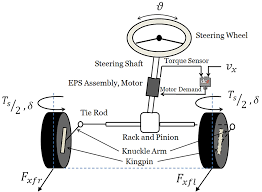
\includegraphics[height=3.5cm]{figs/img/autonomousVehiclesSteering}
    \caption{}
    \label{fig:steerSystem}
  \end{subfigure}
  \caption{\subref{fig:fleet} Autonomous vehicle fleet in AutonomouStuff Solutions and \subref{fig:steerSystem} steering model setup (courtesy of AutonomouStuff). }
  \label{fig:AstuffFleetSteeringSetup}
\end{figure}

% \noindent \begin{tiny}
% 	\textsuperscript{a}https://hexagonpositioning.com/pi-brands/autonomoustuff\\\textsuperscript{b}https://www.autonews.com/article/20181105/OEM10/181109921/delphi-s-pace-award-winning-e-steer-an-autonomous-vehicle-building-block
% \end{tiny}

 \section{Literature Review}

 Authors in~\cite{Hussain2011} illustrates identification of multiple-input
 single-output model for maximum power point tracking of photovoltaic system. A
 significant effort was conducted to model the photovoltaic system, where the two inputs were
 Solar irradiance and Cell temperature, and the output was DC current. To model
 this system, Matlab’s System Identification Toolbox was used. In order to
 create different models, they collected and used data from an energy center in
 Malaysia. After generating different models, the authors ended up going with a
 fourth order ARX (also known as ARXQS) model because it was the most accurate,
 with a best fit percentage of 93.42\%. The polynomial model equation for ARX is
 shown below. %
 %
 \begin{align*}
   y(t) + a_1y(t - 1) +...+a_{na}y(t - n_{a}) = b_{1}u_{1}(t-n_{k})+...+b_{nb}u_{nb}(t - n_{k}-n_{b}+1) + e(t), 
 \end{align*}
% 
$y(t)$ is the system output at time $t,$ while $u(t)$ is the input. The noise disturbance of the system is represented by $e(t).$ The variables $na,$ $nb,$ and $nk$ are the system’s number of poles, amount of $b$ parameters, and the samples before the inputs begin to affect the system’s output.



\section{System Identification Preliminaries}

System identification is the process of developing mathematical models for a dynamic system using the measurement of input and output signals of that system. There are many components that are used to accomplish a task that they are assigned without knowing the exact behavior of the system for given input signals. Without knowing the response of this black-box, there could be unexpected consequences from a system. The goal of the system identification methodology is to get an accurate estimation of the system response to any given input. Mathworks' MATLAB has the System Identification Toolbox, where a few existing examples demonstrate the working principle of this toolbox.

\subsection{Example 1: Dealing with Multi-Variable Systems: Identification and Analysis}
\label{sec:sysID-Example1}

The example given in~\cite{example1} shows how to create an iddata object from a
dataset in order to get the inputs and the outputs. The next step was to look at
the impulse and step responses in order to learn more about how the inputs and
outputs act. From there the state space model was estimated using the first part
of the given data. This model was compared to the step responses and with the
second part of the data to see if it was a good fit. The model had a best fit
percentage of 83.55\% for the generated voltage data, and a best fit of 39.33\%
for the speed data. The frequency response of the model was estimated with
spectral analysis and bode plots were also created. The tutorial explained that
if the data doesn’t give nice models, then it is best to try out submodels for
the different channels. Two single-input single-output (SISO) models were
created and compared with the existing multiple-input multiple-output (MIMO)
model and the actual data. The Nyquist plots were also compared. Both SISO
models performed well during these comparisons. The next step in the tutorial
was to create a multiple-input single-output (MISO) model in order to get a
model that more accurately reflected the generated voltage data. By creating
this model and comparing it to the validation data and previous models, we saw a
best fit percentage of 90.18\%. The last thing the example showed was how to
merge the two SISO models we created earlier.

\begin{figure}[h]
    \centering
    \captionsetup{justification=centering, margin=3cm}
    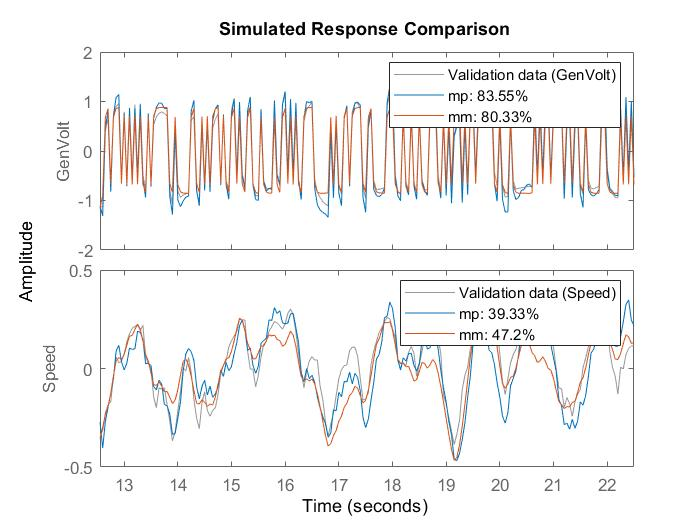
\includegraphics[width=2.5in]{figs/img/mimoExGrady}
    \caption{Comparison of the state space model and merged SISO models with the validation data}
    \label{fig:exMIMO}
\end{figure}

\subsection{Example 2: Selecting Model Structures for Multivariable Systems}
\label{sec:sysID-Example2}
This example~\cite{Matlab2}, discusses solutions for modeling both MISO and MIMO models using Mathworks' Matlab System Identification Toolbox. As the article discusses, MISO system models are easier to develop because all model structures used by the toolbox support models with a single output and multiple inputs. Therefore, the process for developing a model for a MISO system is importing the data as an iddata object, removing the mean from the data, and estimating the solution using any model structure available in the toolbox. The command line can be used by using the function associated with the model structure name and then using the compare function to get the best fit percentage. For MIMO systems, there are not model structures built into the System Identification Toolbox and they must be imported instead. Otherwise the process is very similar to that of a MISO system. For a MIMO system, using the compare function can be crucial. The compare function will tell which output channel is the most difficult to develop a model for, if it is possible at all. With this information, the output channel that is hardest to model should first be modeled individually because there will be less freedom in what model structures are available. The other channels should be able to closely relate to the model for the output channel you selected.

\begin{figure}[htbp]
  \centering
  \begin{subfigure}[b]{0.48\linewidth}
    \centering
    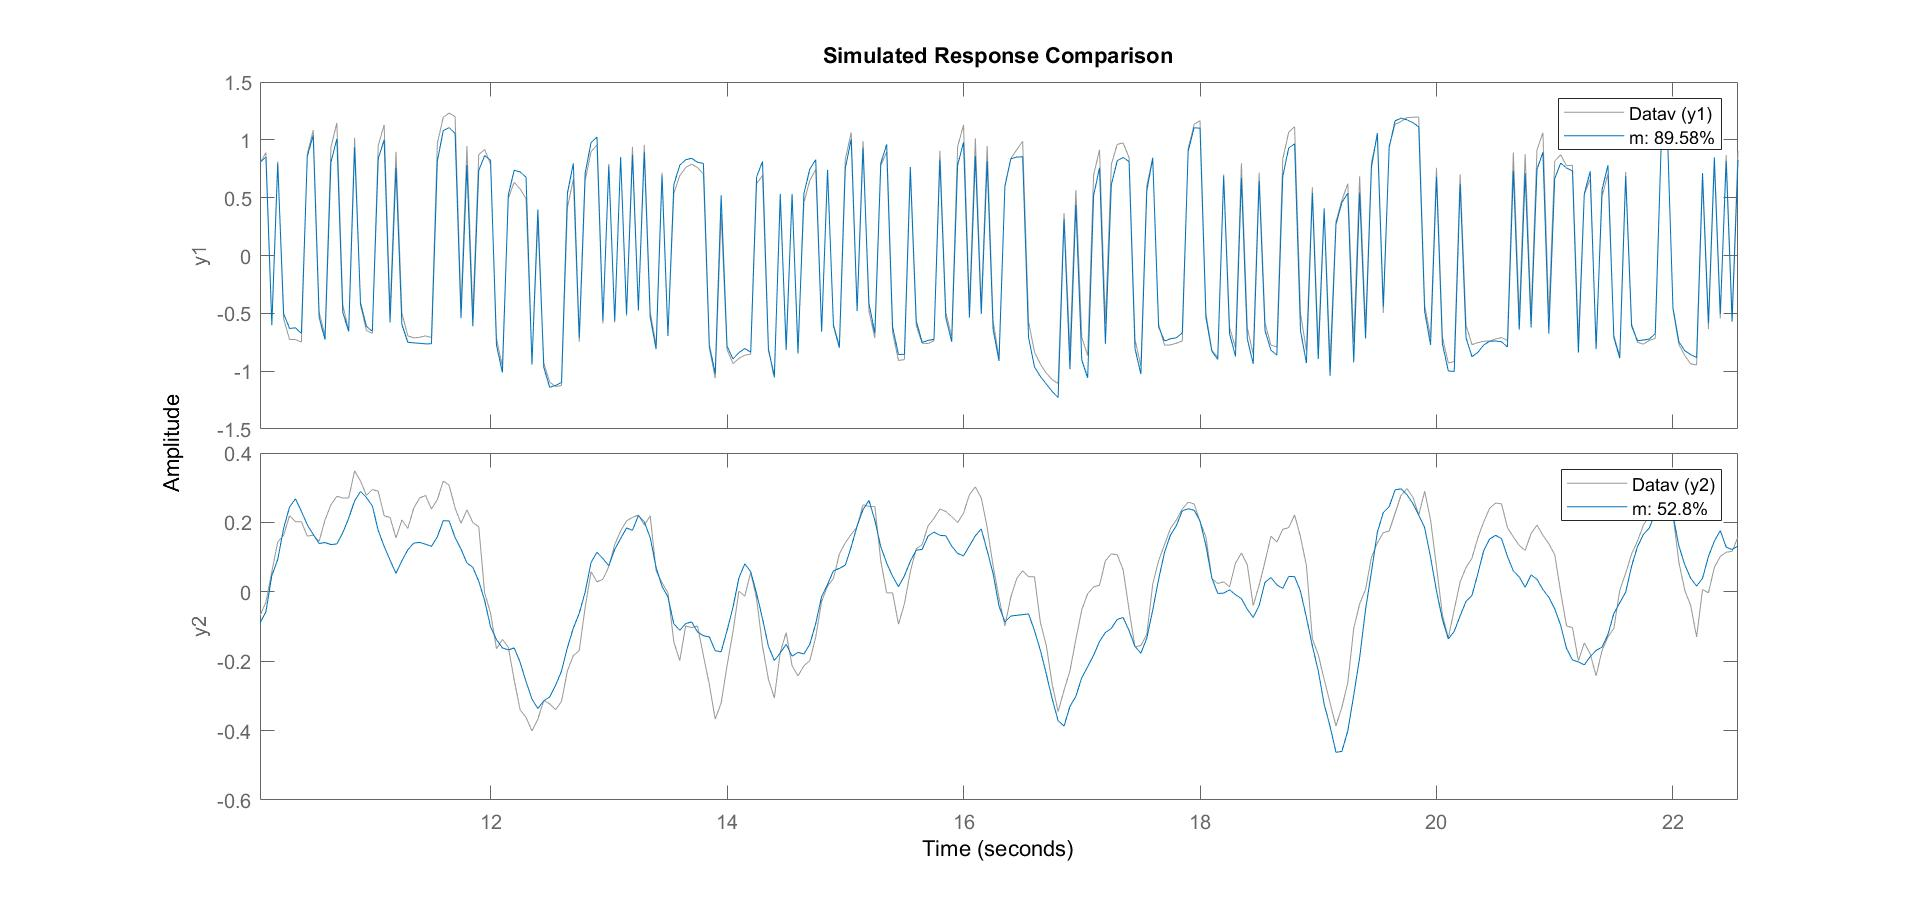
\includegraphics[height=5cm]{figs/img/example2Fig1}
    \caption{}
    \label{fig:ex2fig1}
  \end{subfigure}
  \begin{subfigure}[b]{0.48\linewidth}
    \centering
    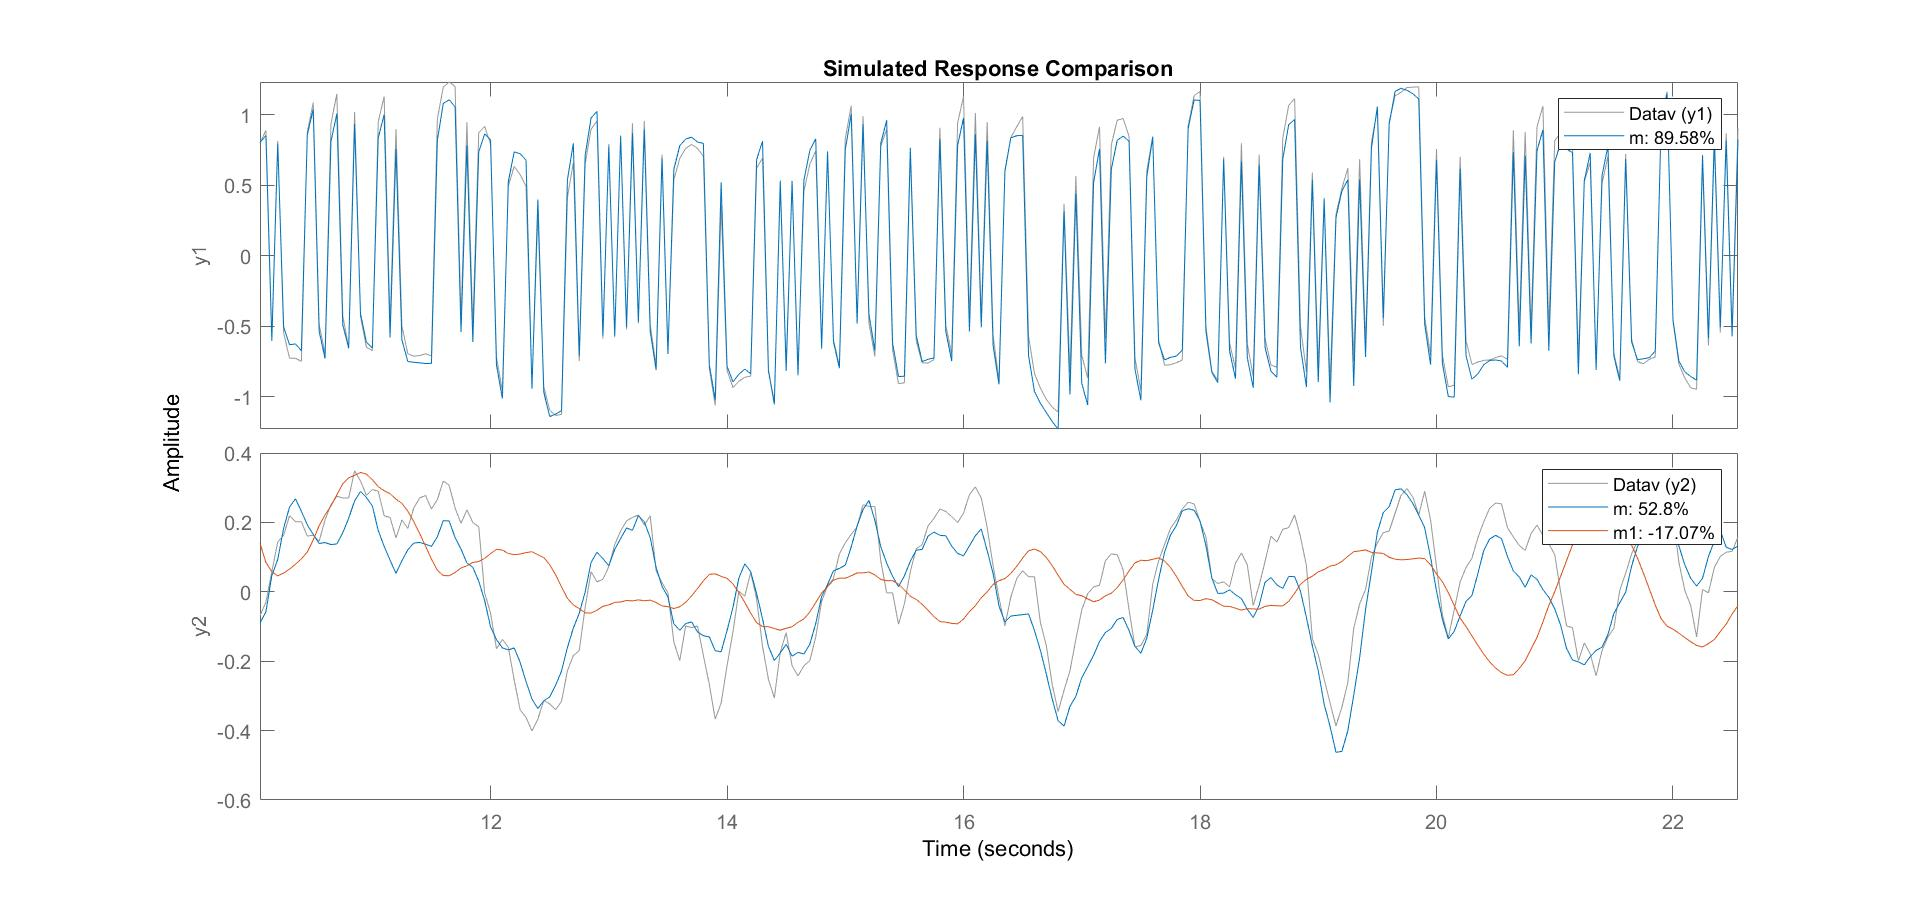
\includegraphics[height=5cm]{figs/img/example2Fig2}
    \caption{}
    \label{fig:ex2fig2}
  \end{subfigure}
  \caption{\subref{fig:ex2fig1} State-space model of a MIMO system with a validation data comparison and \subref{fig:ex2fig2} State-space model of a MIMO system and system-sized based state-space model with a validation data comparison }
  \label{fig:AstuffFleetSteeringSetup}
\end{figure}

\subsection{Example 3: Identify Linear Models Using the Command Line}
\label{sec:sysID-Example3}
This example in~\cite{example3} shows how to create models for MISO systems
using the command line. Before starting the model estimation process, the
equilibrium values of the inputs and outputs had to be taken out. The data from
each experiment also had to be separated into different iddata objects. The
example showed how to estimate and compare non-parametric impulse response,
transfer function, ARMA, state-space, and Box-Jenkins models with the measured
experimental data. The state-space model with the five-step response prediction
was the most accurate, with a best fit percentage of 85.83\%.
\begin{figure}[h]
    \centering
    \captionsetup{justification=centering, margin=3cm}
    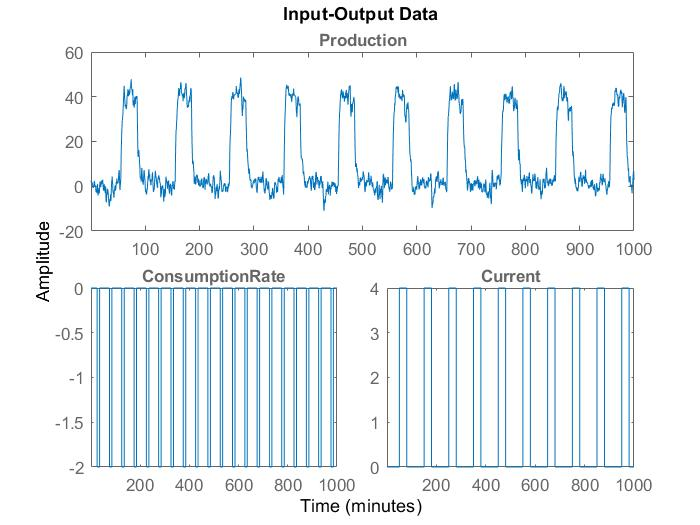
\includegraphics[width=2.5in]{figs/img/commandLineIO}
    \caption{Inputs and outputs of the given system}
    \label{fig:exIO}
\end{figure}


\section{System Requirements}
The vehicle plant model will fulfill the requirements listed below:
\begin{itemize}
    \item The resulting plant model will consist of accurate subsystem models
    \item The subsystems can be used to create an HIL testbench
    \item The steering model can handle very small changes in steering angles
    \begin{itemize}
    		\item The steering model should have a very smooth, continuous output as a choppy, discontinuous output would translate into difficulty tracking the vehicle in a straight line for instances such as keeping the vehicle in its lane. For this reason, that model that we create should be able to smooth out any discontinuities that would normally be measured by the steering motor, especially for small changes in the steering angle. The non-linear behavior is depicted in \autoref{fig:nonlinGraph}.
    \end{itemize}
\end{itemize}
\begin{figure}[h]
    \centering
    \captionsetup{justification=centering, margin=3cm}
    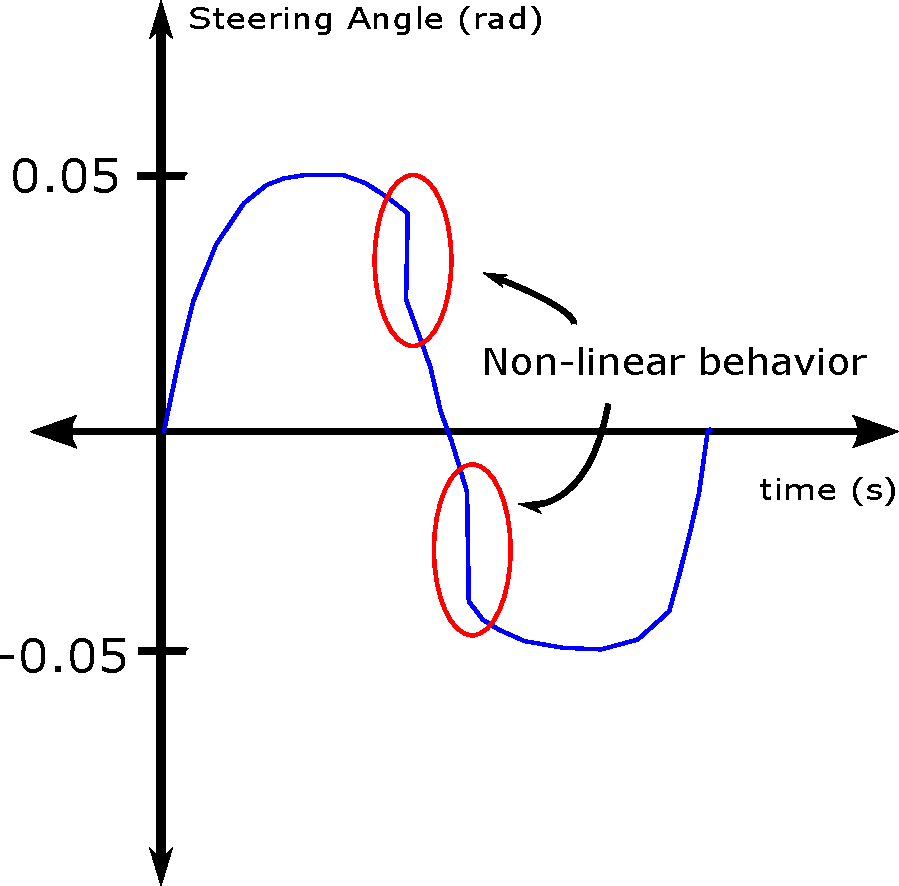
\includegraphics[width=2.5in]{figs/inkscape/nonlinearBehavior}
    \caption{Steering Non-linear Behavior}
    \label{fig:nonlinGraph}
\end{figure}


\section{System Architecture}
The overall system architecture of this project consists of six subsystems which are the steering, acceleration, brake, speed, shift, and speed control systems. Each of the six subsystems can be described as a multiple input system because there are two torque voltage signals used to describe the behavior of each vehicle subsystem. Some of the systems are multiple output and some are single output.

 \subsection{Steering Subsystem}
In addition to the block diagram shown in \autoref{fig:steeringmodelarchitecture}, $\theta_r{}_e{}_f$ ref represents the desired steering wheel angle. This desired angle is entered by the user. $\theta$, the actual steering wheel angle, is subtracted from the desired steering wheel angle to find the error between the two positions. This error value is sent to the steering subsystem’s controller. Using this information, the controller generates torque voltages A and B, which are sent to the steering subsystem. New torque voltages are then generated and the actual steering wheel angle is updated. 

 \begin{figure}[h]
    \centering
    \captionsetup{justification=centering, margin=3cm}
    \includegraphics[width=2.5in]{figs/inkscape/steeringmodelarchitecture}
    \caption{Steering subsystem block diagram}
    \label{fig:steeringmodelarchitecture}
\end{figure}

 \begin{figure}[h]
    \centering
    \captionsetup{justification=centering, margin=3cm}
    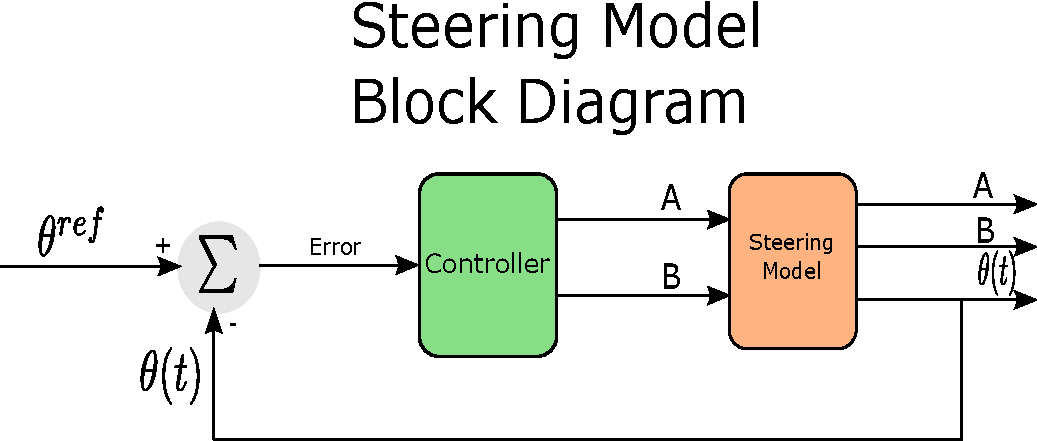
\includegraphics[width=2.5in]{figs/inkscape/steeringModelBlockDiagram}
    \caption{Steering block diagram}
    \label{fig:steeringModelBlockDiagram}
\end{figure}
  
  \subsection{Brake Subsystem}
  The brake subsystem takes the Brake Pedal Pressure Voltages, Brake Pedal Stroke Voltages, and the Brake Pedal On/Off Switch values as inputs. Using these values, it generates a new Brake Pedal Position and a boolean value called Brake Pressed. This boolean value indicates to the user whether or not the brake pedal is being pressed. The brake subsystem is another example of a multiple-input multiple-output system. 
 \begin{figure}[h]
    \centering
    \captionsetup{justification=centering, margin=3cm}
    \includegraphics[width=2.5in]{figs/inkscape/brakeModelArchitecture}
    \caption{Brake subsystem block diagram}
    \label{fig:brakeModelArchitecture}
\end{figure}
 
  \subsection{Acceleration Subsystem}
  The acceleration subsystem is a multiple-input multiple-output system. 
Acceleration pedal voltages are sent to the subsystem. 
A new acceleration pedal position value is generated to better match 
the real-time pedal position. This is then the output 
of the acceleration subsystem.
 \begin{figure}[h]
    \centering
    \captionsetup{justification=centering, margin=3cm}
    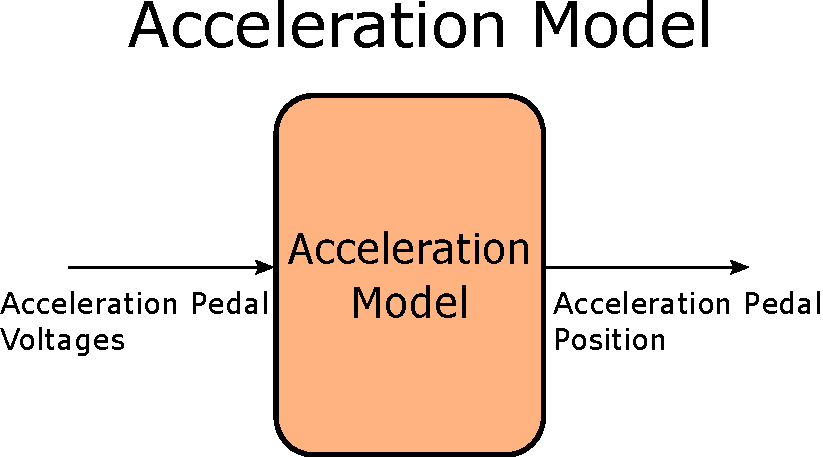
\includegraphics[width=2.5in]{figs/inkscape/accelerationModelArchitecture}
    \caption{Acceleration subsystem block diagram}
    \label{fig:accelerationModelArchitecture}
\end{figure}
 
  \subsection{Shift Subsystem}
 This subsystem can be classified as a single-input single-output system. The subsystem takes the desired shifter gear value from the user. Within the subsystem, the actual shifter gear changes to better reflect the desired gear. This actual shifter gear value is then the output of the shift subsystem. 
 \begin{figure}[h]
    \centering
    \captionsetup{justification=centering, margin=3cm}
    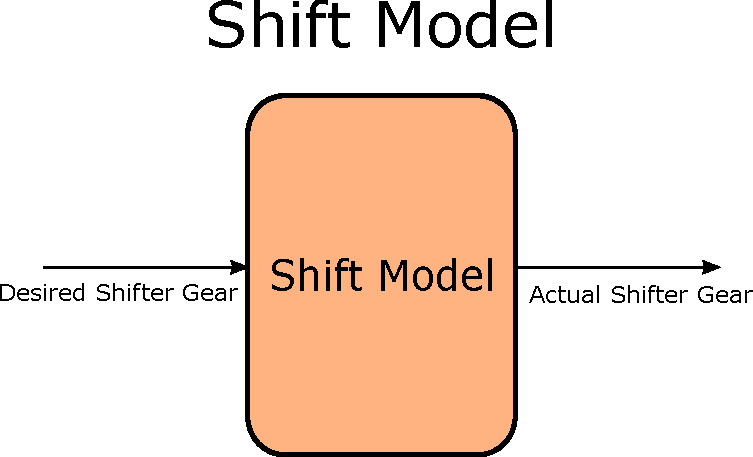
\includegraphics[width=2.5in]{figs/inkscape/shiftModelArchitecture}
    \caption{Shift subsystem block diagram}
    \label{fig:shiftModelArchitecture}
\end{figure}
 
  \subsection{Speed Subsystem}
This speed subsystem would fall under the multiple-input single-output system. There are four inputs, the position of the acceleration pedal and the brake pedal, along with the shifter actual gear. Taking these inputs, the speed subsystem finds the vehicle speed. This vehicle speed is the output of the system.  
 \begin{figure}[h]
    \centering
    \captionsetup{justification=centering, margin=3cm}
    \includegraphics[width=2.5in]{figs/inkscape/speedModelArchitecture}
    \caption{Speed subsystem block diagram}
    \label{fig:speedModelArchitecture}
\end{figure}
 
  \subsection{Speed Control Subsystem}
  The speed control subsystem is a straightforward single-input single-output system. The desired vehicle speed is set by the user and sent to the speed control subsystem. Taking this input, the subsystem calculates the new vehicle speed. This value is then sent out to the rest of the vehicle system. 
 \begin{figure}[h]
    \centering
    \captionsetup{justification=centering, margin=3cm}
    \includegraphics[width=2.5in]{figs/inkscape/speedControlModelArchitecture}
    \caption{Speed Control subsystem block diagram}
    \label{fig:speedControlModelArchitecture}
\end{figure}

%\begin{figure}[htb]
%    \centering 
%\begin{subfigure}[b]{0.48\linewidth}
%  \centering 
%  \includegraphics[width=2.5in]{figs/inkscape/steeringmodelarchitecture}
%  \caption{}
%  \label{fig:steeringmodelarchitecture}
%\end{subfigure}
%\begin{subfigure}[b]{0.48\linewidth}
%  \centering
%  \includegraphics[width=2.5in]{figs/inkscape/brakeModelArchitecture}
%  \caption{}
%  \label{fig:brakeModelArchitecture}
%\end{subfigure}
%\\
%\begin{subfigure}[b]{0.48\textwidth}
%  \centering 
%  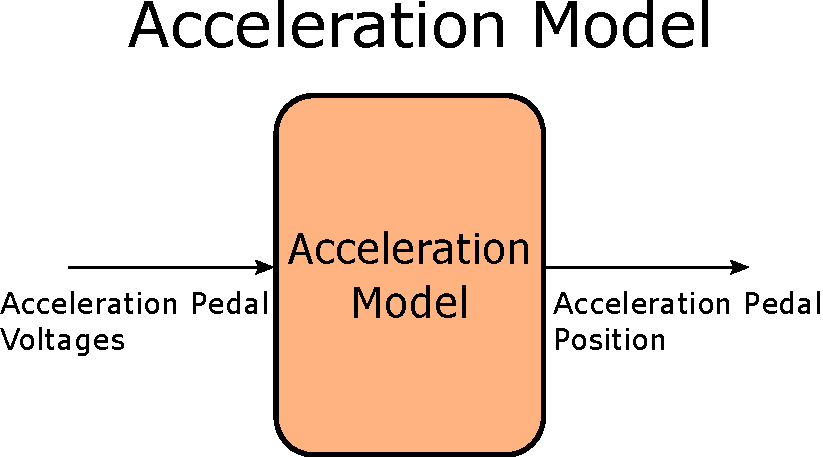
\includegraphics[width=2.5in]{figs/inkscape/accelerationModelArchitecture}
%  \caption{}
%  \label{fig:accelerationModelArchitecture}
%\end{subfigure}
%\begin{subfigure}[b]{0.48\linewidth}
%  \centering 
%  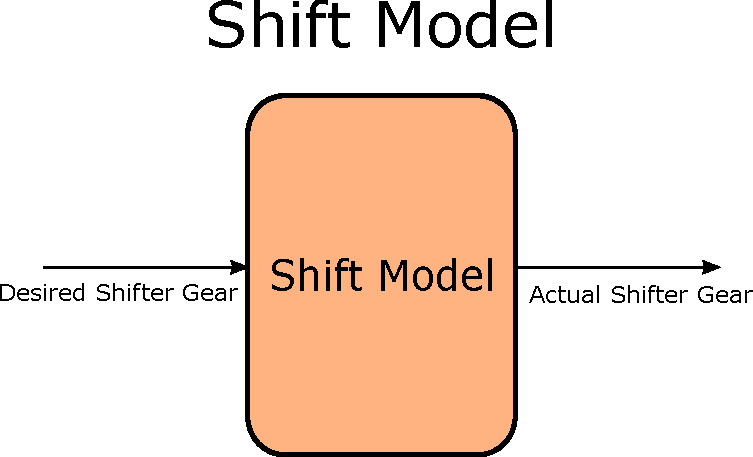
\includegraphics[width=2.5in]{figs/inkscape/shiftModelArchitecture}
%  \caption{}
%  \label{fig:shiftModelArchitecture}
%\end{subfigure}
%\\
%\begin{subfigure}[b]{0.48\linewidth}
%  \centering
%  \includegraphics[width=2.5in]{figs/inkscape/speedControlModelArchitecture}
%  \caption{}
%  \label{fig:speedControlModelArchitecture}
%\end{subfigure}
%\begin{subfigure}[b]{0.48\linewidth}
%  \centering
%  \includegraphics[width=2.5in]{figs/inkscape/speedModelArchitecture}
%  \caption{}
%  \label{fig:speedModelArchitecture}
%\end{subfigure}
%\caption{Block diagrams of autonomous vehicle subsystems:~\subref{fig:steeringmodelarchitecture} steering subsystem,~\subref{fig:brakeModelArchitecture} brake subsystem,~\subref{fig:accelerationModelArchitecture} acceleration subsystem,~\subref{fig:shiftModelArchitecture} shift subsystem,~\subref{fig:speedControlModelArchitecture} speed control subsystem, and~\subref{fig:speedModelArchitecture} speed subsystem.}
%\label{fig:subFunctionalBlock}
%\end{figure}


 \subsection{Specifications}
 Based on the system requirements listed above, the plant model will meet the following specifications:
 \begin{itemize}
    \item The steering subsystem will be modeled first due to its non-linearities, depicted in \autoref{fig:nonlinGraph}, and because it is important to the operation of the vehicle 
    \item The steering subsystem will be able to handle small steering angles
    \item Each vehicle subsystem will be modeled separately
 \end{itemize}

\section{Main Project Work (Modeling Vehicle Subsystems)}
To start this project, we first read documentation outlining the uses of MATLAB's System Identification Toolbox. From there we worked on MATLAB tutorials on how to model systems from data using System Identification and then find the most accurate model. We specifically tried to find examples with Multiple-Input Multiple-Output (MIMO) and Multiple-Input Single-Output (MISO) systems, since most of the vehicle subsystems we will model fall into one of these categories. A literature review was also conducted to see how systems with small non-linearities like our steering subsystem were modeled using System Identification. On October 7th we traveled to AutonomouStuff in order to collect data from the steering, acceleration, and braking subsystems in an autonomous vehicle. The data we collected will be used to generate and then verify our models. We collected data on the Lexus RX450H vehicle platform shown in \autoref{fig:exusvehicle}. 


\begin{figure}[h]
	\centering
	\captionbox{AutonomouStuff Lexus RX450H Vehicle}
	{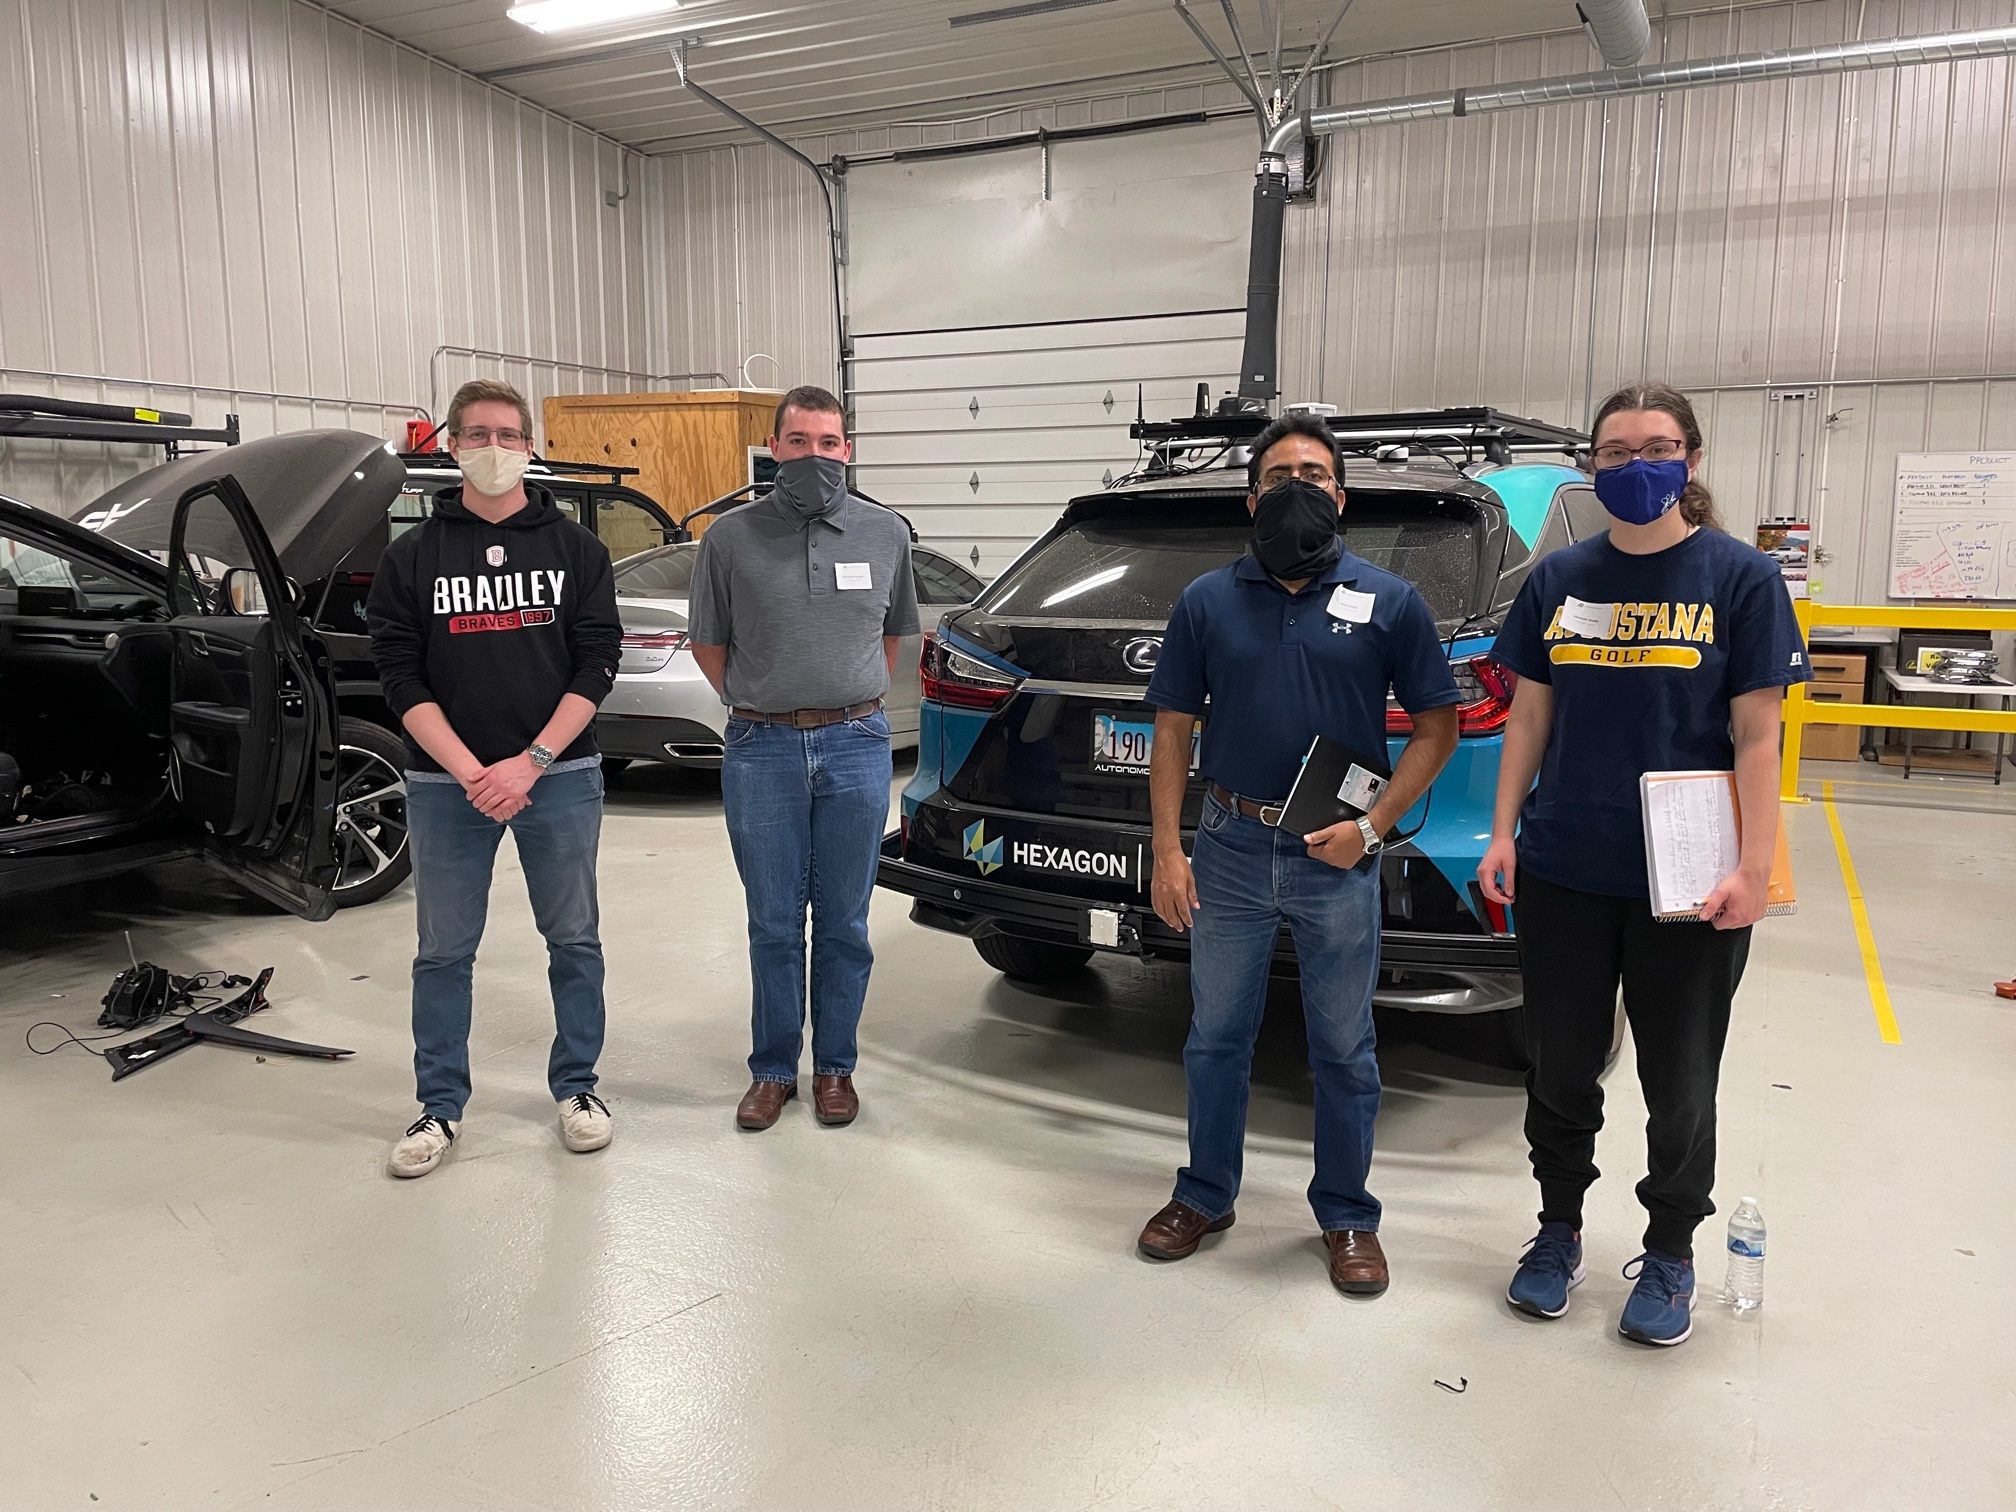
\includegraphics[height=3.5cm, width=0.4\linewidth]{figs/img/picturesVisitToAStuff/visitors1-20211007}}
	\label{fig:lexusvehicle}
\end{figure}


\noindent The following is the hardware required for this project:  
	\begin{itemize}
    		\item Laptop
    		\item PACMod ECU
    		\item CANCase 
    		\item CAN bus 
 	\end{itemize}
 	
 	
	\noindent The laptop is used to pass commands or log data, such as steering angle or acceleration or brake pedal position. This data is sent or received using the CANCase and CAN bus. These are connected to the AutonomouStuff designed PACMod ECU, which sends torque voltages to the desired vehicle subsystem allowing the laptop to either control the desired vehicle system or log data.\bigskip

	\noindent The following is the software required for this project: 
	\begin{itemize}
    		\item MATLAB's System Identification Toolbox 
    		\item Vector CANAlyzer 
 	\end{itemize}
 	
 	
 	\noindent The Vector CANAlyzer software is installed on the laptop and is used to parse the collected data that is sent from the CANCase. This is how we were able to collect logs of data that we would use to develop models of the autonomous vehicle subsystems. MATLAB's System Identification Toolbox is the software that gave us the capabilities to develop these models of the vehicle subsystems. Using this toolbox, we are able to use the logs of data we collected to create sets of estimation and validation data that will be used for training the model.


\noindent Each subsystem that we are modeling is set up in a similar manner. In manual mode, the torque voltages that control each subsystem are sent by the vehicle's electronic control unit (ECU). In order to control the vehicle autonomously, the vehicle subsystem switches to by-wire mode. In by-wire mode, the torque voltages from the vehicle's ECU are discarded by open-circuiting the motors that control each subsystem. Instead, the PACMod ECU built by AutonomouStuff sends the torque voltages to the motor using relays. In \autoref{fig:vehicleSetup}, the experimental setup for data collection is shown. The laptop is used to collect the data from the desired vehicle subsystem by the use of Vector's CANAlyzer software. The CAN Case collects data from the PAC Mod and ECU and sends the data using a CAN bus to the laptop which is then parsed and displayed through the use of CANAlyzer. The ECU and PAC Mod are not shown in \autoref{fig:vehicleSetup} as they are fixed behind panels of the vehicle. 

\begin{figure}
	\centering
    	\captionsetup{justification=centering, margin=3cm}
    	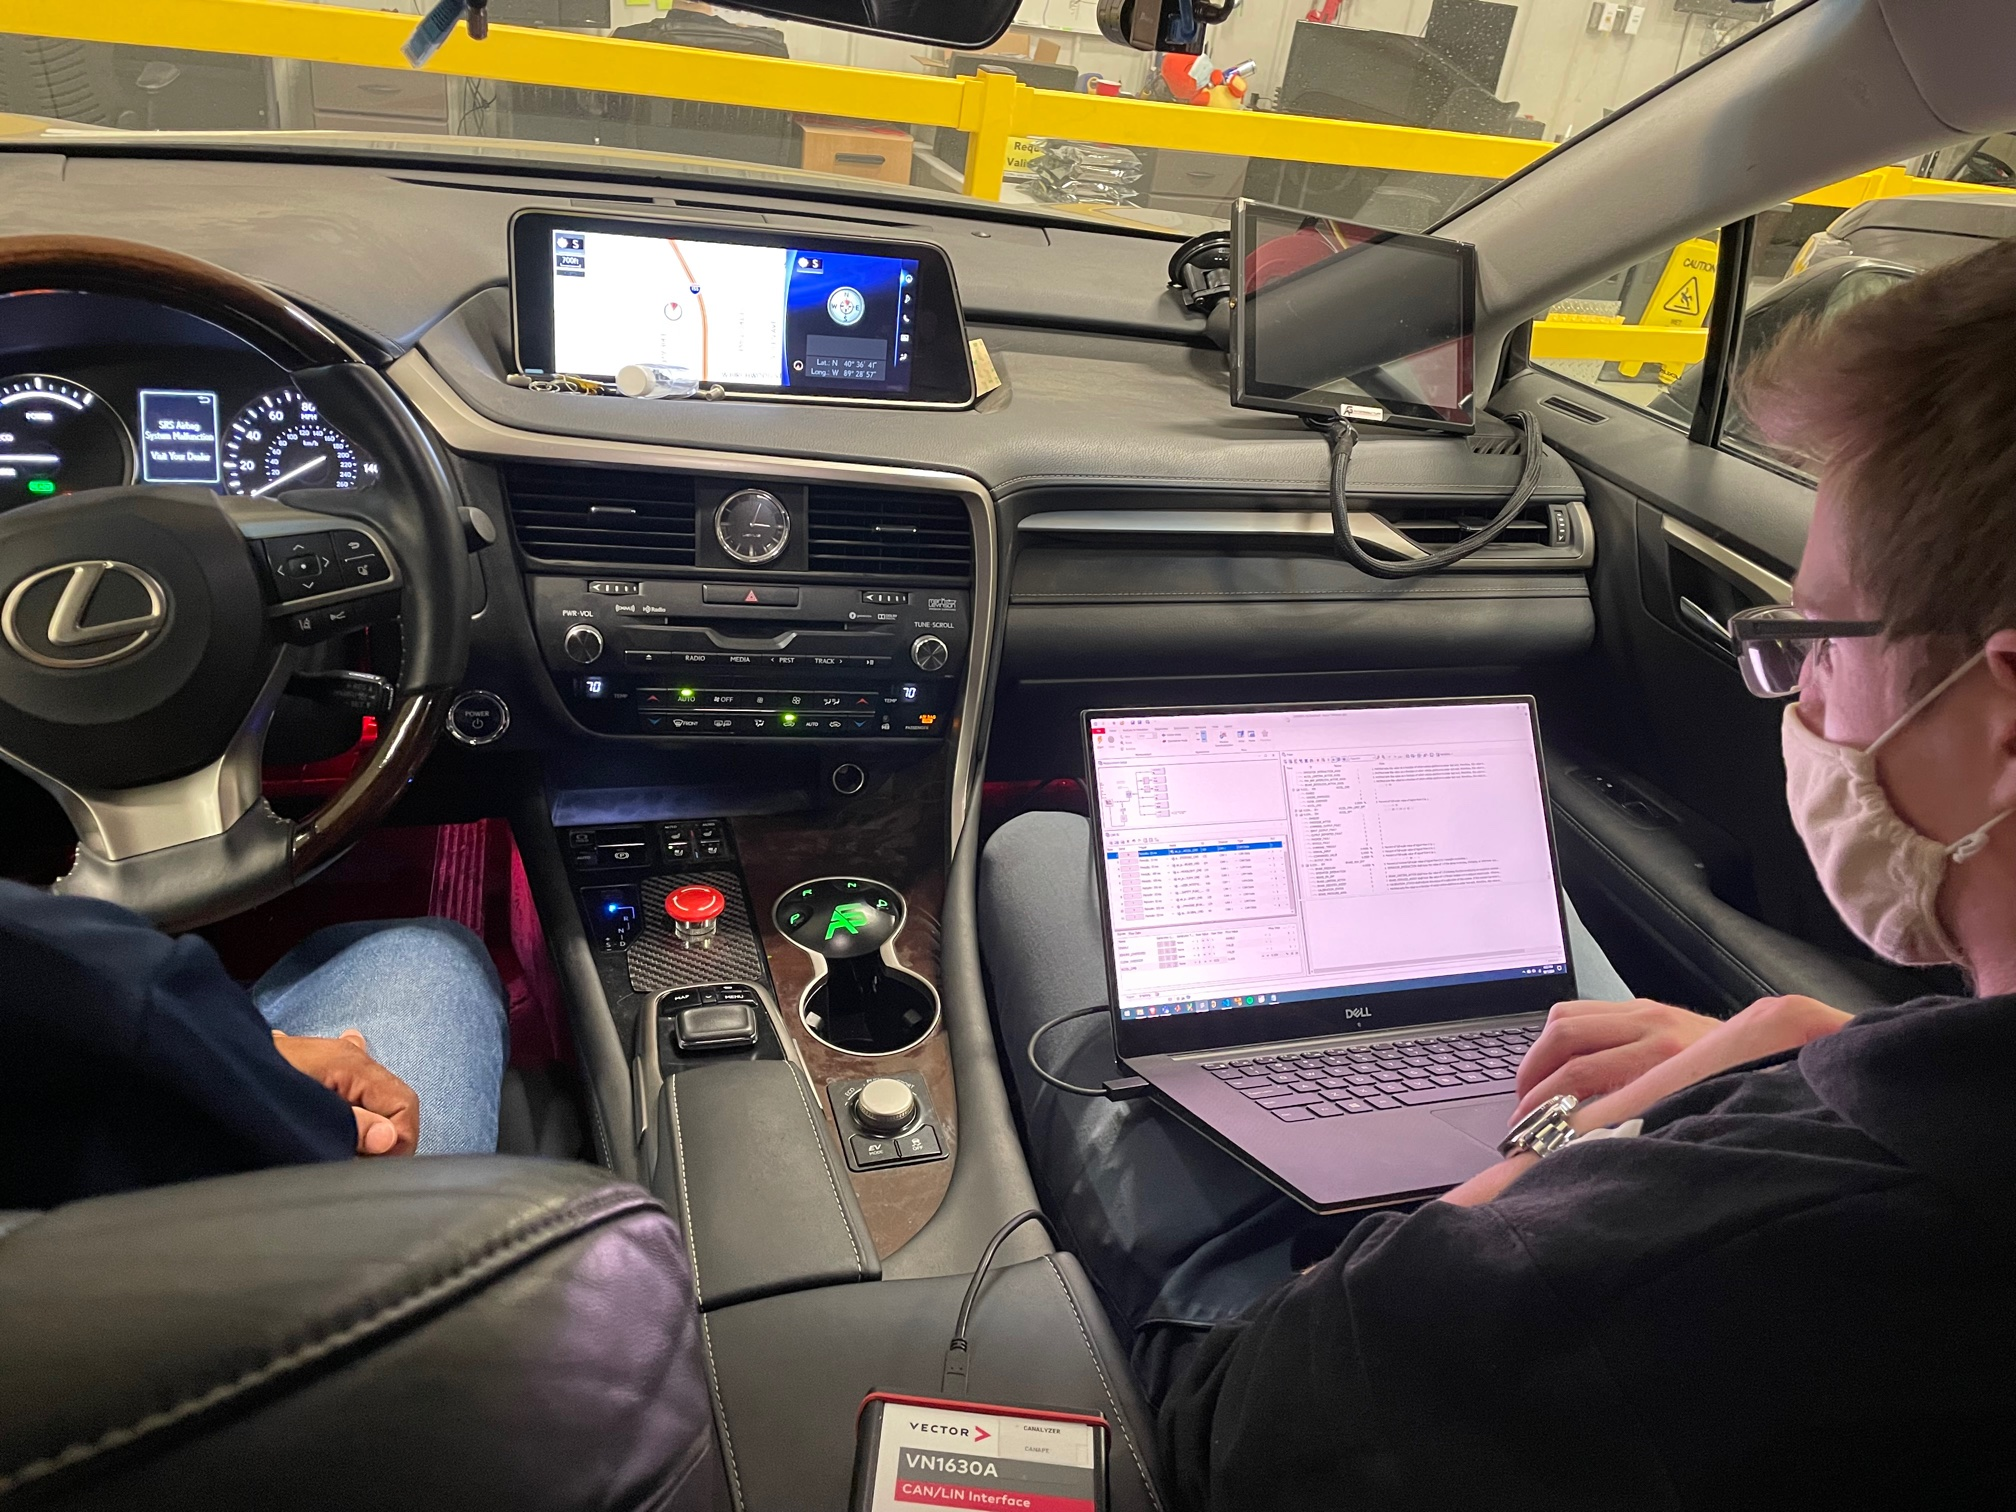
\includegraphics[width=5in]{figs/img/picturesVisitToAStuff/dataColletionSetup1-20211007}
    	\caption{Autonomous Vehicle Data Collection Setup}
    	\label{fig:vehicleSetup}
\end{figure}

\section{Validation and Testing} \label{sec:simresults}
\subsection{Steering System}
In \autoref{byWireSteerModel}, the output steering angle is plotted versus time when the vehicle is in by-wire mode. The figure shows the output steering angle from some data collected to depict the steering system behavior plotted with the behavior of the estimated model. The best fit percentage for this model is 85.54\%. Likewise, \autoref{manualSteerModel} depicts the output steering angle plotted versus time when the vehicle is in manual mode. The best fit percentage for this model is 90.27\%. 


  % %
  % \begin{figure}
  %   \centering
  %   \begin{subfigure}[b]{0.48\linewidth}
  %     \centering
  %     \includegraphics[width=\textwidth]{figs/fusion360/PowertrainModelCorrectDimsTopViewV3}
  %     \caption{}
  %     \label{fig:PowertrainModelCorrectDimsTopViewV3}
  %   \end{subfigure}
  %   \begin{subfigure}[b]{0.48\linewidth}
  %     \centering
  %     \includegraphics[width=\textwidth]{figs/fusion360/PowertrainModelCorrectDimsFrontViewV4}
  %     \caption{}
  %     \label{fig:PowertrainModelCorrectDimsFrontViewV4}
  %   \end{subfigure}
  %   \begin{subfigure}[b]{0.48\linewidth}
  %     \centering
  %     \includegraphics[width=\textwidth]{figs/fusion360/PowertrainModelCorrectDimsSideViewV4}
  %     \caption{}
  %     \label{fig:PowertrainModelCorrectDimsSideViewV4}
  %   \end{subfigure}
  %   \caption{\subref{fig:PowertrainModelCorrectDimsTopViewV3} Top view,
  %     \subref{fig:PowertrainModelCorrectDimsFrontViewV4} front view, and
  %     \subref{fig:PowertrainModelCorrectDimsSideViewV4} side view of the
  %     proposed disinfecting robot.}
  %   \label{fig:2dViewsDisinfectingRobot}
  % \end{figure}

\begin{figure}[h]
	\centering
	\subcaptionbox{Output of Estimated By-Wire System Model \label{byWireSteerModel}}
		{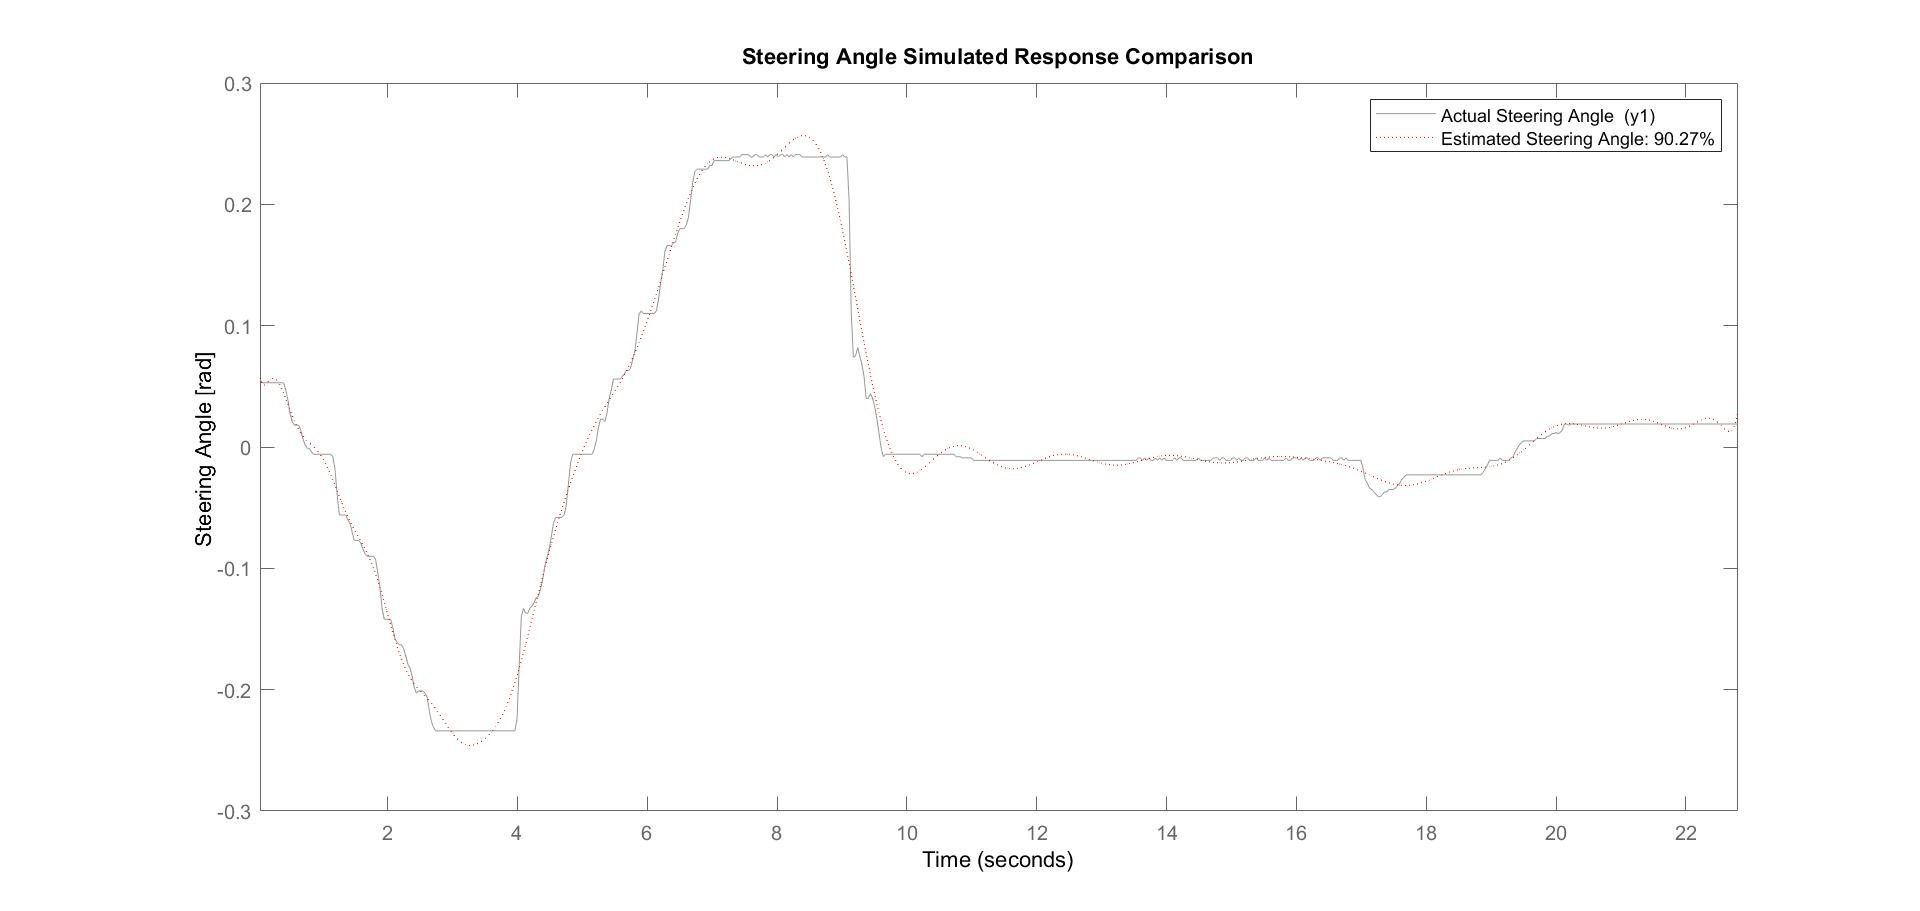
\includegraphics[width=0.48\linewidth]{figs/img/byWireSteeringTransferFunctionModel}}
	\subcaptionbox{Output of Estimated Manual System Model \label{manualSteerModel}}
		{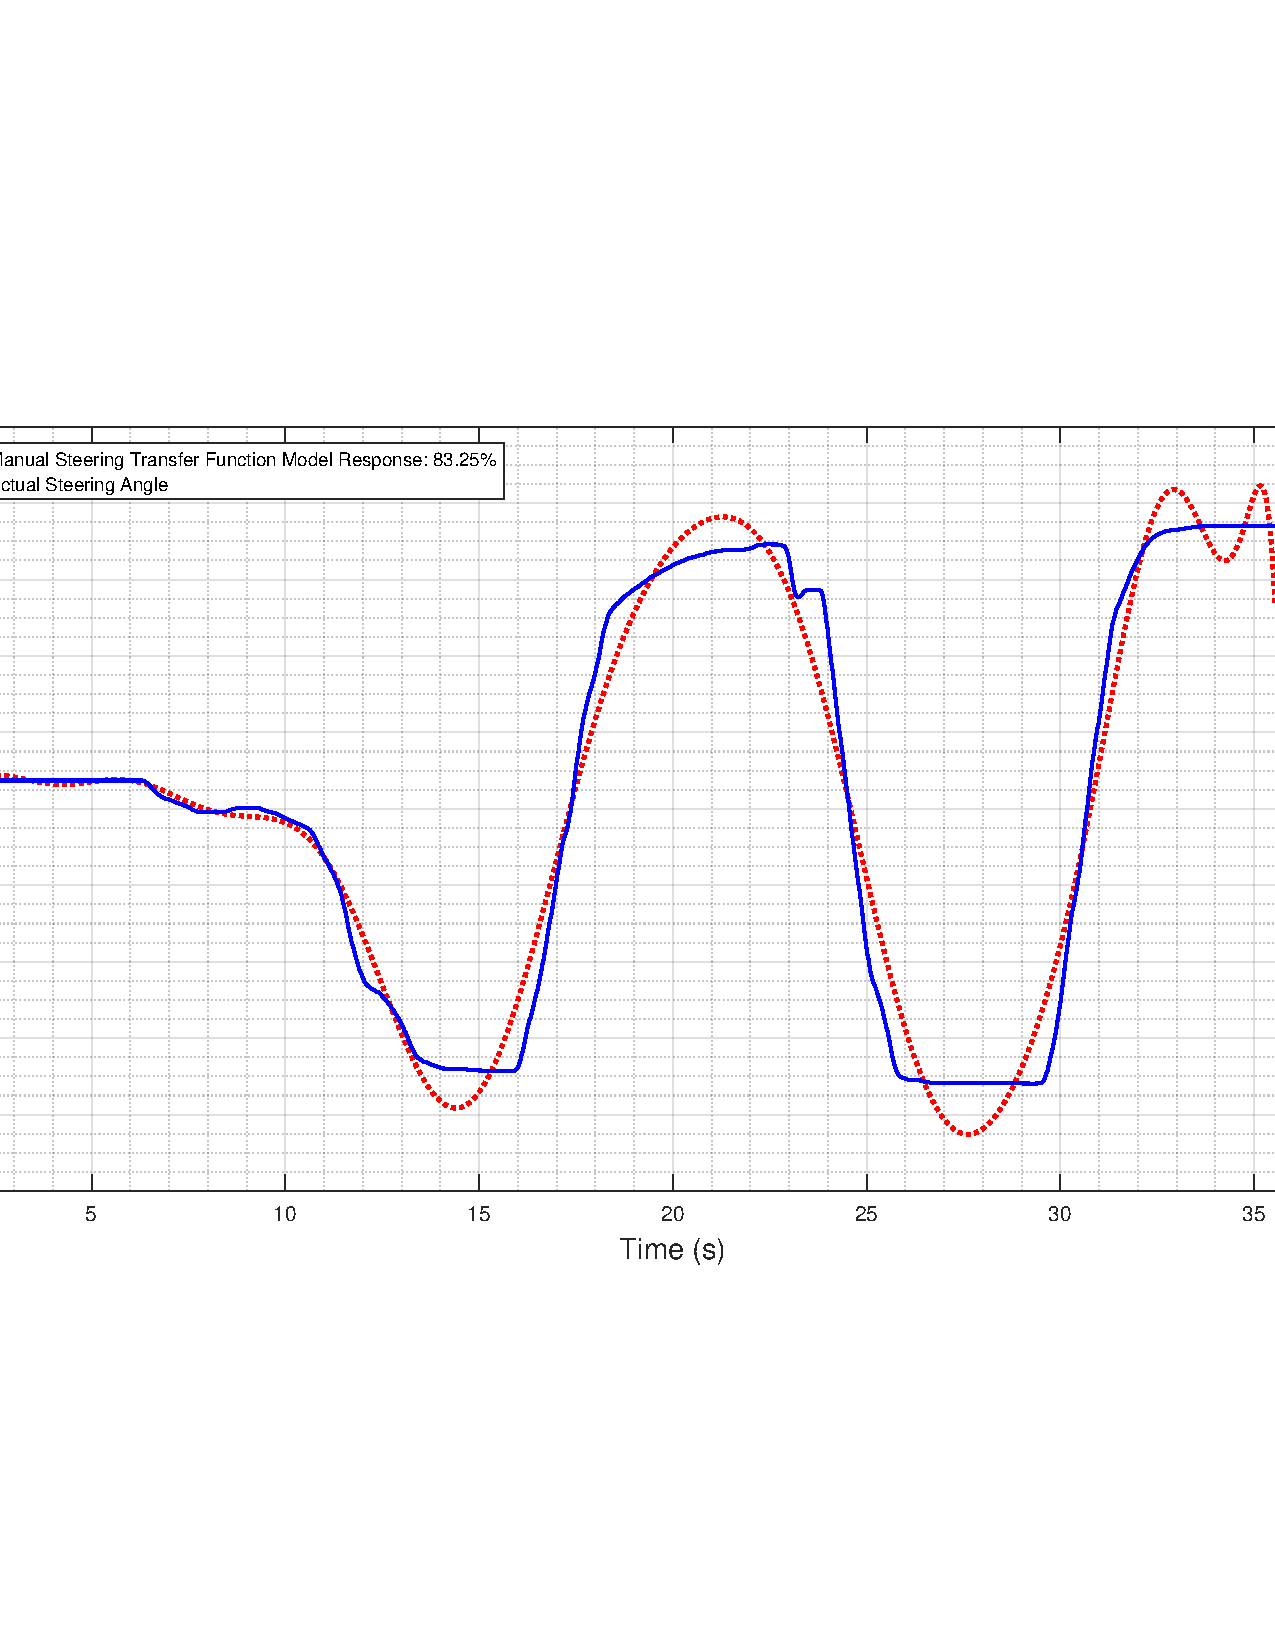
\includegraphics[width=0.48\linewidth]{figs/img/manualSteeringTransferFunctionModel}}
	\caption{Steering System Estimated Steering Angle Comparison}
\end{figure}

\vspace{12pt}
\noindent The model of the by-wire steering system is a twentieth order transfer function. The twentieth order transfer function is the best proposed estimation considering the system costs associated with a higher order transfer function while also obtaining an acceptable best fit percentage. \autoref{tab:byWireSteerCoeffA} shows the coefficients of the twentieth order transfer function for the output steering angle with respect to the input torque voltage A signal.%
%
\begin{table}[hbtp]
	\label{tab:byWireSteerCoeffA}
	\caption{By-Wire Mode Steering Transfer Function Torque Voltage A Coefficient Table}
  \centering
  \resizebox{\linewidth}{!}{% Resize table to fit within \linewidth horizontally
    \begin{tabular}{*{21}{c}}
      \toprule
      $a_0$& $a_1$&$a_2$&$a_3$&$a_4$&$a_5$&$a_6$&$a_7$&$a_8$&$a_9$&$a_{10}$&$a_{11}$&$a_{12}$&$a_{13}$&$a_{14}$&$a_{15}$&$a_{16}$&$a_{17}$&$a_{18}$ &$a_{19}$&$a_{20}$\\
      \midrule
      1.949E-16 & 1.455E-14 & 8.797E-13 & 2.304E-11 & 9.041E-10 & 9.01E-9 & 2.714E-7 & 9.241E-7 & 1.946E-5 & 3.889E-5 & 0.0005721 & 0.0008035 & 0.008695 & 0.008922 & 0.07499 & 0.05422 & 0.3631 & 0.1693 & 0.9394 & 0.2118 & 1\\
      \bottomrule
    \end{tabular}}
    
	\begin{center}
		\resizebox{0.4\linewidth}{!}{% Resize table to fit within \linewidth horizontally
    		\begin{tabular}{*{21}{c}}
      	\toprule
      	$b_0$& $b_1$&$b_2$&$b_3$&$b_4$&$b_5$\\
      	\midrule
      	3.44E-16 & -2.203E-15 & 1.24E-13 & 5.975E-13 & 3.001E-12 & 5.23E-12\\
      	\bottomrule
    		\end{tabular}}
	\end{center}	
\end{table}
%
 
\noindent \autoref{tab:byWireSteerCoeffB} shows the coefficients of the twentieth order transfer function for the output steering angle with respect to the input torque voltage B signal.%
%
\begin{table}[hbtp]
	\label{tab:byWireSteerCoeffB}
	\caption{By-Wire Mode Steering Transfer Function Torque Voltage B Coefficient Table}
  \centering
  \resizebox{\linewidth}{!}{% Resize table to fit within \linewidth horizontally
    \begin{tabular}{*{21}{c}}
      \toprule
      $a_0$& $a_1$&$a_2$&$a_3$&$a_4$&$a_5$&$a_6$&$a_7$&$a_8$&$a_9$&$a_{10}$&$a_{11}$&$a_{12}$&$a_{13}$&$a_{14}$&$a_{15}$&$a_{16}$&$a_{17}$&$a_{18}$ &$a_{19}$&$a_{20}$\\
      \midrule
      2.92E-15 & 2.758E-13 & 1.761E-11 & 4.228E-10 & 1.422E-8 & 1.561E-7 & 1.501E-6 & 8.426E-6 & 5.981E-5 & 0.0002016 & 0.001226 & 0.002649 & 0.01456 & 0.02044 & 0.104 & 0.09228 & 0.4417 & 0.2257 & 1.025 & 0.2305 & 1\\
      \bottomrule
    \end{tabular}}
	\begin{center}
		\resizebox{0.4\linewidth}{!}{% Resize table to fit within \linewidth horizontally
    		\begin{tabular}{*{21}{c}}
     	 \toprule
     	 $b_0$& $b_1$&$b_2$&$b_3$&$b_4$&$b_5$\\
     	 \midrule
      	-6.645E-15 & 2.161E-14 & -2.605E-14 & -4.744E-13 & -1.813E-13 & -4.858E-12\\
      	\bottomrule
    \end{tabular}}
	\end{center}
\end{table}
%

\vspace{12pt}
\noindent The manual steering system is modeled by a twentieth order transfer
function. After considering the system costs that come with a higher order
transfer function and the need to achieve a sufficient best fit percentage, it
is clear that a twentieth order transfer function is the best estimation of the
system. \autoref{tab:manualSteerCoeffA} shows the coefficients of the twentieth
order transfer function for the output steering angle with respect to the input
torque voltage A signal. %
%
  \begin{table}[hbtp]
    \caption{Manual mode steering transfer function torque voltage A coefficient table. }
    \label{tab:manualSteerCoeffA}
    \centering
	  \resizebox{\linewidth}{!}{% Resize table to fit within \linewidth horizontally
      \begin{tabular}{*{21}{c}}
        \toprule
        $a_0$& $a_1$&$a_2$&$a_3$&$a_4$&$a_5$&$a_6$&$a_7$&$a_8$&$a_9$&$a_{10}$&$a_{11}$&$a_{12}$&$a_{13}$&$a_{14}$&$a_{15}$&$a_{16}$&$a_{17}$&$a_{18}$ &$a_{19}$&$a_{20}$\\
        \midrule
        1.224E5 & 4.227E5 & 2.202E6 & 3.54E6 & 7.98E6 & 7.62E5 & 1.071E7 & 6.745E6 & 6.85E6 & 3.006E6 & 2.365E6 & 7.37E5 & 4.669E5 & 1.021E5 & 5.319E4 & 7752 & 3353 & 287.5 & 102.4 & 3.653 & 1\\
        \bottomrule
      \end{tabular}}
    \begin{center}
    	\resizebox{0.4\linewidth}{!}{% Resize table to fit within \linewidth horizontally
        \begin{tabular}{*{21}{c}}
          \toprule
          $b_0$& $b_1$&$b_2$&$b_3$&$b_4$&$b_5$\\
          \midrule
          6.516E4 & -2.944E5 & 2.328E5 & -2.487E5 & 8.25E4 & -3.038E4\\
          \bottomrule
        \end{tabular}}
    \end{center}
  \end{table}
%


\noindent \autoref{tab:manualSteerCoeffB} shows the coefficients of
the twentieth order transfer function for the output steering angle with respect
to the input torque voltage B signal. %
%
\begin{table}[hbtp]
	\caption{Manual Mode Steering Transfer Function Torque Voltage B Coefficient Table}
	\label{tab:manualSteerCoeffB}
  \centering
  \resizebox{\linewidth}{!}{% Resize table to fit within \linewidth horizontally
    \begin{tabular}{*{21}{c}}
      \toprule
      $a_0$& $a_1$&$a_2$&$a_3$&$a_4$&$a_5$&$a_6$&$a_7$&$a_8$&$a_9$&$a_{10}$&$a_{11}$&$a_{12}$&$a_{13}$&$a_{14}$&$a_{15}$&$a_{16}$&$a_{17}$&$a_{18}$ &$a_{19}$&$a_{20}$\\
      \midrule
      4.687E4 & 7.037E5 & 2.624E6 & 6.133E6 & 1.197E7 & 1.487E7 & 1.887E7 & 1.446E7 & 1.314E7 & 7.01E6 & 4.79E6 & 1.886E6 & 9.836E5 & 2.937E5 & 1.149E5 & 2.617E4 & 7205 & 1232 & 200 & 23.54 & 1\\
      \bottomrule
    \end{tabular}}
	\begin{center}
    \resizebox{0.4\linewidth}{!}{% Resize table to fit within \linewidth horizontally
      \begin{tabular}{*{21}{c}}
        \toprule
        $b_0$& $b_1$&$b_2$&$b_3$&$b_4$&$b_5$\\
        \midrule
        1.209E4 & 1.855E5 & -2.801E5 & 4.72E5 & -3.976E4 & 7.693E4\\
        \bottomrule
      \end{tabular}}
	\end{center}	
\end{table}
%

\subsection{Acceleration System}
In \autoref{byWireAccelModel}, the output acceleration pedal position is plotted versus time when the vehicle is in by-wire mode. The figure shows the output acceleration pedal position from some data collected to depict the acceleration system behavior plotted with the behavior of the estimated model. The best fit percentage for this model is 97.69\%. Likewise, \autoref{manualAccelModel} depicts the output acceleration pedal position plotted versus time when the vehicle is in manual mode. The best fit percentage for this model is 98.3\%. 

\begin{figure}[h]
	\centering
	\subcaptionbox{Output of Estimated By-Wire System Model \label{byWireAccelModel}}
		{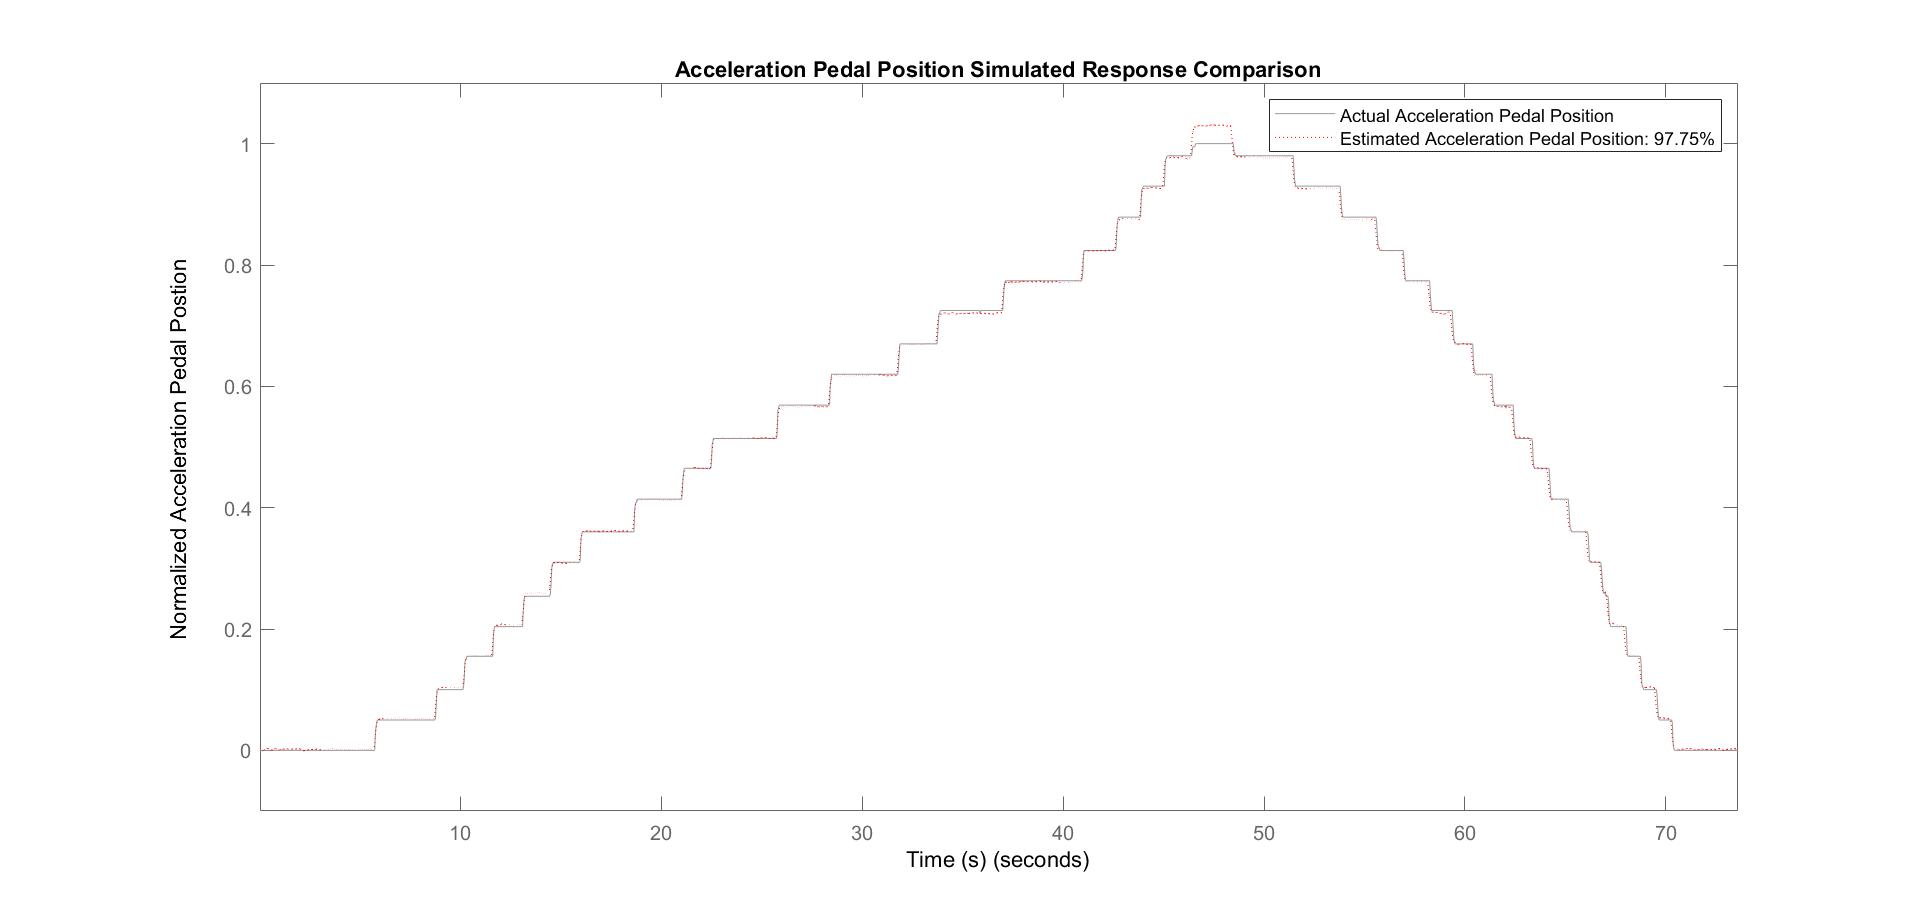
\includegraphics[width=0.48\linewidth]{figs/img/byWireAccelArxModel}}
	\subcaptionbox{Output of Estimated Manual System Model \label{manualAccelModel}}
		{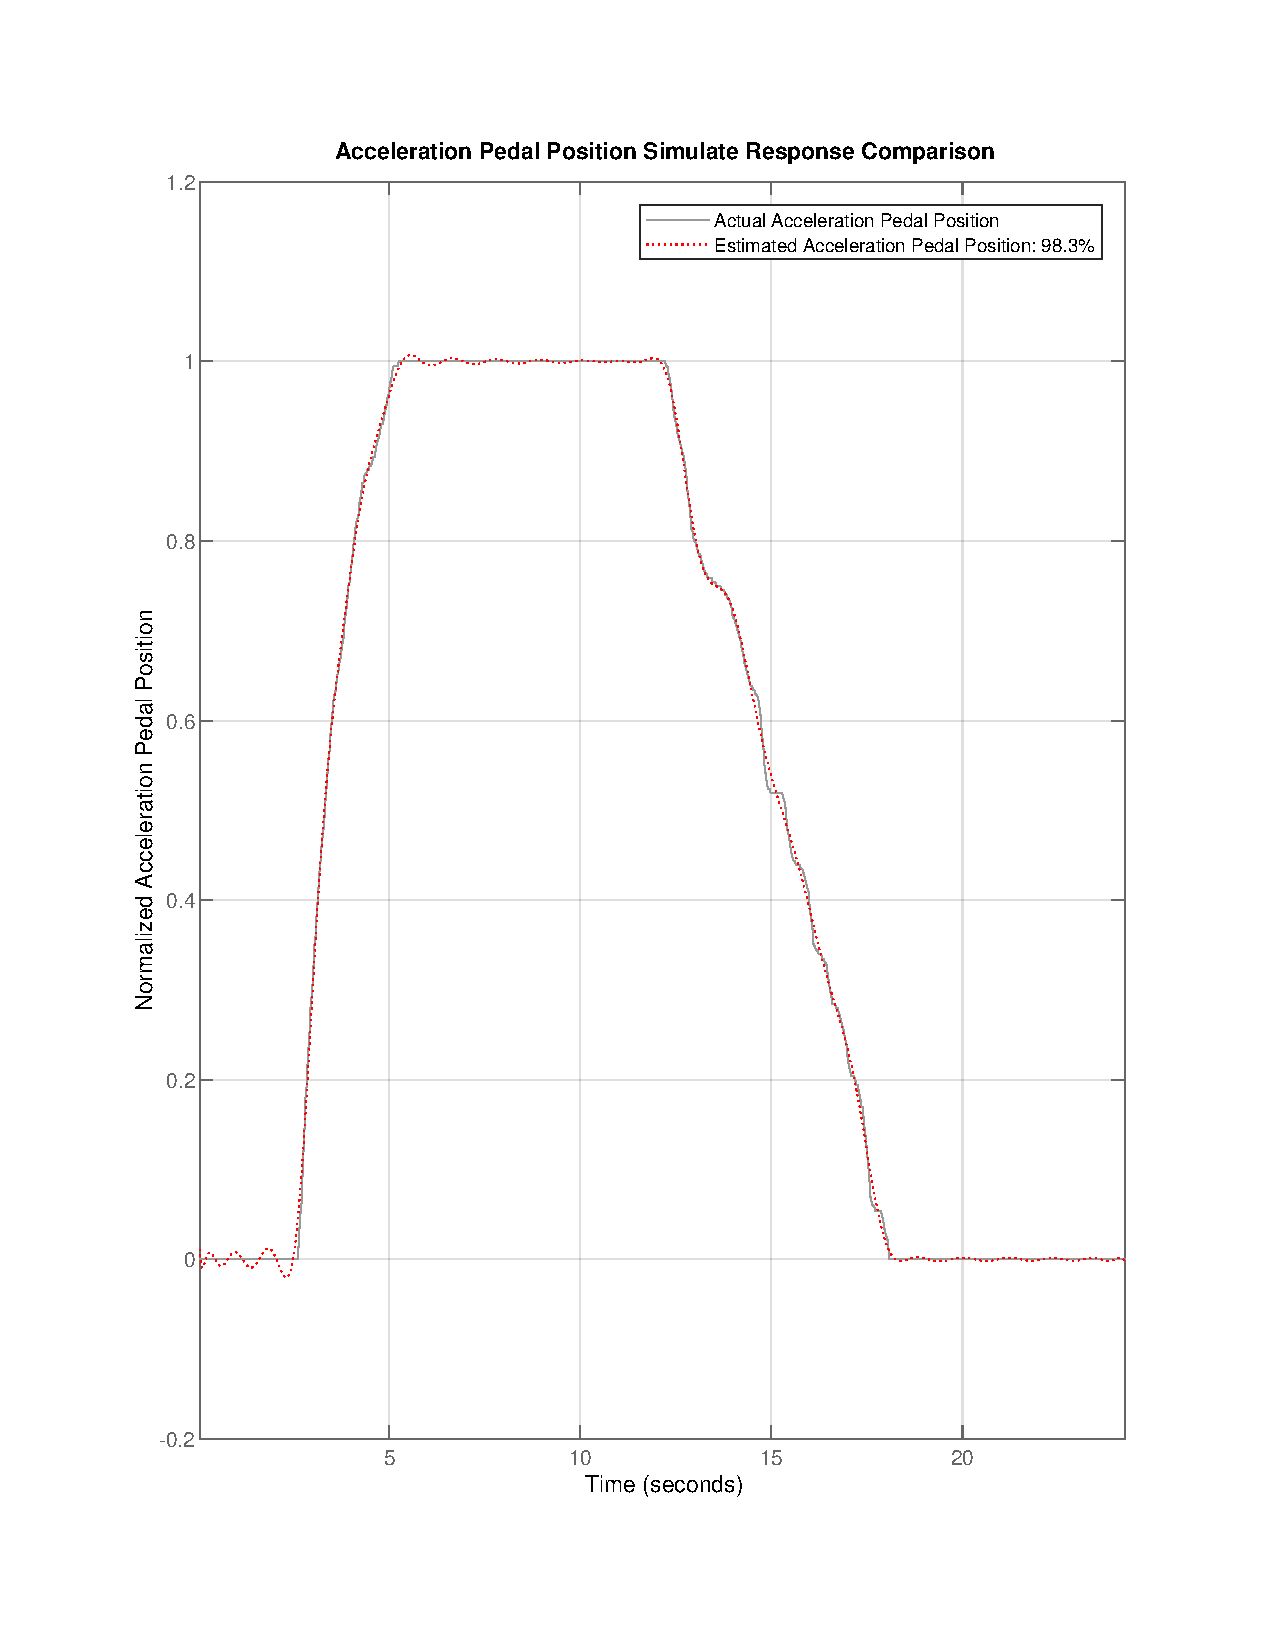
\includegraphics[width=0.48\linewidth]{figs/img/manualAccelTransferFunctionModel}}
	\caption{Acceleration System Estimated Pedal Position Comparison}
\end{figure}

\vspace{12pt}
\noindent The model of the by-wire acceleration system is a fourth order ARX model. The fourth order ARX model defined below represents the output acceleration pedal position, A(z), based on input torque voltage A, $B_1(z)$, and input torque voltage B, $B_2(z)$. 
% 
	\begin{align*}
		A(z)y(t) &= B_1(z)u_1(t) + B_2(z)u_2(t) + e(t),
	\end{align*}
	%
	where na = 4, nb = 4, nk = 0, and, 
	%
  \begin{align*}
		A(z) &= 1 - 1.018z^{-1} - 0.002901z^{-2} + 0.4631z^{-3} - 0.2038z^{-4}\\
    B_1(z) &= -0.0207 - 0.01912z^{-1} - 0.02159z^{-2} - 0.03307z^{-3}\\
		B_2(z) &= 0.02017 + 0.01833z^{-1} + 0.09461z^{-2} + 0.05683z^{-3}
  \end{align*}
%

\vspace{12pt}
\noindent The model of the manual acceleration system is a twenty-fourth order transfer function. The twenty-fourth order transfer function is the best proposed estimation considering the system costs associated with a higher order transfer function while also obtaining an acceptable best fit percentage. \autoref{tab:manualAccelCoeffA} shows the coefficients of the twenty-fourth order transfer function for the output acceleration pedal position with respect to the input torque voltage A signal. %
%
\begin{table}[hbtp]
	\caption{Manual Mode Acceleration Transfer Function Torque Voltage A Coefficient Table}
	\label{tab:manualAccelCoeffA}
  \centering
  \resizebox{\linewidth}{!}{% Resize table to fit within \linewidth horizontally
    \begin{tabular}{*{25}{c}}
      \toprule
      $a_0$& $a_1$&$a_2$&$a_3$&$a_4$&$a_5$&$a_6$&$a_7$&$a_8$&$a_9$&$a_{10}$&$a_{11}$&$a_{12}$&$a_{13}$&$a_{14}$&$a_{15}$&$a_{16}$&$a_{17}$&$a_{18}$ &$a_{19}$&$a_{20}$&$a_{21}$&$a_{22}$&$a_{23}$&$a_{24}$\\
      \midrule
      2.307E7 & 8.369E7 & 9.137E8 & 1.992E9 & 3.753E9 & 5.454E9 & 5.548E9 & 5.869E9 & 3.453E9 & 3.161E9 & 1.54E9 & 9.654E8 & 3.556E8 & 1.789E8 & 5.082E7 & 2.071E7 & 4.569E6 & 1.498E6 & 2.553E5 & 6.532E4 & 8443 & 1559 & 147.3 & 15.5 & 1\\
      \bottomrule
    \end{tabular}}
    \begin{center}
    		\resizebox{0.4\linewidth}{!}{% Resize table to fit within \linewidth horizontally
    \begin{tabular}{*{7}{c}}
      \toprule
      $b_0$& $b_1$&$b_2$&$b_3$&$b_4$&$b_5$&$b_6$\\
      \midrule
      -5.741E6 & -2.644E7 & -2.797E6 & -1.304E7 & -3.203E6 & -1.159E6 & -5.519E5\\
      \bottomrule
    \end{tabular}}
    \end{center}
\end{table}
%

\noindent \autoref{tab:manualAccelCoeffB} shows the coefficients of the twenty-fourth order transfer function for the output acceleration pedal position with respect to the input torque voltage B signal.%
%
\begin{table}[hbtp]
	\caption{Manual Mode Acceleration Transfer Function Torque Voltage B Coefficient Table}
	\label{tab:manualAccelCoeffB}
  \centering
  \resizebox{\linewidth}{!}{% Resize table to fit within \linewidth horizontally
    \begin{tabular}{*{25}{c}}
      \toprule
      $a_0$& $a_1$&$a_2$&$a_3$&$a_4$&$a_5$&$a_6$&$a_7$&$a_8$&$a_9$&$a_{10}$&$a_{11}$&$a_{12}$&$a_{13}$&$a_{14}$&$a_{15}$&$a_{16}$&$a_{17}$&$a_{18}$ &$a_{19}$&$a_{20}$&$a_{21}$&$a_{22}$&$a_{23}$&$a_{24}$\\
      \midrule
      5.224E6 & 4.205E7 & 1.429E8 & 3.233E8 & 5.444E8 & 7.326E8 & 8.247E8 & 7.402E8 & 6.301E8 & 3.99E8 & 2.731E8 & 1.264E8 & 7.223E7 & 2.48E7 & 1.216E7 & 3.084E6 & 1.324E6 & 2.422E5 & 9.264E4 & 1.159E4 & 4003 & 307.4 & 96.87 & 3.451 & 1\\
      \bottomrule
    \end{tabular}}
    \begin{center}
    	\resizebox{0.4\linewidth}{!}{% Resize table to fit within \linewidth horizontally
    \begin{tabular}{*{7}{c}}
      \toprule
      $b_0$& $b_1$&$b_2$&$b_3$&$b_4$&$b_5$&$b_6$\\
      \midrule
      -4.159E6 & 1.851E6 & -4.457E6 & 9.043E5 & -7.45E5 & 1.865E5 & -1.545E4\\
      \bottomrule
    \end{tabular}}
    \end{center}	
\end{table}
%


\section{Timeline and Milestones} \label{sec:timeline}


The Gantt chart highlighting the progress and potential schedule of the project in Fall 2021 is shown in Figure~\ref{fig:gantt1}.  

 \begin{figure}
   \centering
   \begin{ganttchart}[
     hgrid,
     vgrid,
     x unit=.6cm,
     y unit title=.8cm,
     y unit chart=.6cm,
     milestone label font=\tiny,
     milestone progress label font = \tiny,
     milestone progress label anchor = east,
     bar label font=\tiny,
     group label font=\small,
     bar/.append style={fill=green},
     bar incomplete/.append style={fill=red},
     group progress label font = \tiny,
     progress label text={$\displaystyle#1\%$},
     group progress label anchor = east,
     bar progress label font = \tiny,
     bar progress label anchor = east,
     ]{1}{17}

%     \gantttitle{2020}{17}\\
     \gantttitle{Sep}{4}
     \gantttitle{Oct}{4}
     \gantttitle{Nov}{4}
     \gantttitle{Dec}{4}
     \gantttitle{}{1}\\

%     \ganttgroup[progress = 100]{Research}{3}{12} \\
     \ganttbar[progress = 100]{Read System Identification Documentation}{3}{6}\\
     \ganttbar[progress = 100]{Collect Steering, Acceleration, and Braking Data}{6}{7}\\

%     \ganttgroup[progress = 80]{Simulation}{8}{10}\\
     \ganttbar[progress = 100]{System Identification Tutorials}{4}{7}\\
     \ganttbar[progress = 100]{System Functional Requirements Document}{4}{9}\\
          \ganttbar[progress = 100]{System Functional Requirements Presentation}{4}{9}\\

     \ganttbar[progress = 100]{Parts Order Request}{8}{12}\\
     \ganttbar[progress = 100]{Proposal Document}{9}{15}\\
     \ganttbar[progress = 100]{Proposal Presentation}{9}{15}\\

%     \ganttgroup[progress = 82.5]{XBee Setup}{13}{14}\\
     \ganttmilestone[progress = 100]{Model Steering System}{13}{14}\\
     \ganttbar[progress = 100]{Model Acceleration System}{14}{15}\\
     \ganttbar[progress = 100]{Model Braking System}{15}{15}\\
     
   \end{ganttchart}
 \caption{Gantt chart for Fall 2021}
 \label{fig:gantt1}
 \end{figure}



The potential schedule for our project in Spring 2022 is highlighted in the gantt chart shown in Figure~\ref{fig:gantt2}. 
 

 
 \begin{figure}
   \centering
   \begin{ganttchart}[
     hgrid,
     vgrid,
     x unit=.6cm,
     y unit title=.8cm,
     y unit chart=.6cm,
     milestone label font=\tiny,
     milestone progress label font = \tiny,
     milestone progress label anchor = east,
     bar label font=\tiny,
     group label font=\small,
     bar/.append style={fill=green},
     bar incomplete/.append style={fill=red},
     group progress label font = \tiny,
     progress label text={$\displaystyle#1\%$},
     group progress label anchor = east,
     bar progress label font = \tiny,
     bar progress label anchor = east,
     ]{1}{18}
     %\gantttitle{2021}{18}\\
     \gantttitle{Jan}{2}
     \gantttitle{Feb}{4}
     \gantttitle{Mar}{4}
     \gantttitle{Apr}{4}
     \gantttitle{May}{4}\\

%     \ganttgroup[progress = 0]{Assembly}{3}{4}\\
     \ganttbar[progress = 0]{Collect Shift, Speed Control, and Speed Data}{3}{3}\\
     \ganttbar[progress = 0]{Model Shift System}{3}{4}\\
     \ganttbar[progress = 0]{Model Speed Control System}{5}{6}\\
     \ganttbar[progress = 0]{Model Speed System}{7}{8}\\

%     \ganttgroup[progress = 10]{Software}{5}{6}\\
     \ganttbar[progress = 0]{Test Subsystems}{9}{12}\\
     \ganttmilestone[progress = 0]{Test Subsystems with HIL}{12}{15}\\

%     \ganttgroup[progress = 0]{Project Completion}{16}{17}\\
     \ganttmilestone[progress = 0]{Final Report}{15}{15}\\
     \ganttmilestone[progress = 0]{Final Presentation}{16}{16}\\
     \ganttbar[progress = 0]{Presentation to IAB}{17}{17}\\
     \ganttbar[progress = 0]{Project Demo}{17}{17}\\

%     \ganttmilestone[progress = 0]{Project Complete}{17}
   \end{ganttchart}
   \caption{Gantt Chart for Spring 2022}
   \label{fig:gantt2}
 \end{figure}

	Our Gantt charts shown in Figures \ref{fig:gantt1} and \ref{fig:gantt2} outline our project work and milestones for the year. While we are still working on the details, we plan on splitting the work equally to make sure that we each get a chance to learn from this project and to keep it fair for all team members.  


The first milestone on our list will be to model the steering system. This will be a challenge due to its small non-linearities around very small steering angle changes. The next milestone will be to test our subsystem models on AutonomouStuff's HIL system. This is one of the most important milestones because the company sponsors our project and we are working to help solve one of their problems. Our last two milestones will be to present our work in the form of a final report and presentation. This is where all of our work will come together and we will get a chance to explain how we solved the problem. 

We plan on demonstrating our project for AutonomouStuff along with including a full report on how we modeled the vehicle subsystems. As for the final report and presentation, we plan on working on it as soon as possible next semester. This presentation will also be shown to the Industrial Advisory Board. 


% The Gantt charts in Figures \ref{fig:gantt1} and \ref{fig:gantt2} show our planned schedule to complete this project. In these charts, there are four sections in each month represented by the dotted grid. This is to approximate a weekly schedule. Our first milestone is to complete the simulation of the system in MATLAB and CoppeliaSim. This includes simulating a remote as well as the robotic cart. The simulation of the RSSI detection will be handled in Matlab based on the positions of the cart and remote. We will add noise to the simulated RSSI in order to simulate the multipath effect. The expected functionality is that the cart will follow the remote.

% The second milestone is to complete the assembly of both the cart and the remote. The cart assembly involves replacing the existing motors with the purchased motors, as well as mounting the stepper motor, reflector, and XBee on top of the robot. The assembly of the remote involves constructing the voltage regulator circuit.

% The third milestone is to integrate the subsystems into one system. This will involve testing the angle and distance estimation from the cart to the remote. It will also include testing the following capabilities of the overall system. We expect that this will require a large amount of debugging and tuning. Therefore, we have allotted several weeks for this purpose.

% The fourth and final milestone is to complete the final report and presentation. This involves documenting our findings in a report and presenting our work. At this point, the project will be complete.

\section{Concluding Remarks}
Autonomous vehicles have a numerous amount of useful applications in today's society. From being used for delivering packages to allowing drivers to rest while traveling, as the technology for autonomous vehicles is enhanced, they will become an enticing product that many consumers will purchase and use. One of the biggest concerns with autonomous vehicles today is the risk associated with public safety. One solution to reducing the safety risk is ensuring that accurate controllers are developed to reliably control each subsystem involved with the movement of the autonomous vehicle. Due to non-linear behaviors, there is no simple solution for developing reliable controllers. This project will focus on deriving models of some main subsystems so that these non-linear behaviors are removed and smooth controllers can be developed.

\pagebreak
\bibliographystyle{IEEEtran}
\bibliography{bib/references.bib}

\end{document} 

%%% Local Variables:
%%% mode: latex
%%% TeX-master: t
%%% End:
